% Chapter 1: Stochastic processes and stationarity
% Time Series Analysis -- Bachelor's programmes Economic Informatics and Economic Cybernetics, Bucharest University of Economic Studies
% GENERATED by latex/build_chapter1.py -- edit the generator, not this file.

\newcommand{\coursename}{Time Series Analysis}
% Preambul comun TSA -- Serii de timp / Time Series Analysis (Beamer, 16:9)
% Același design ca MFM și SFM (preluat din SFM, 5 octombrie 2026). Înainte de % Preambul comun TSA -- Serii de timp / Time Series Analysis (Beamer, 16:9)
% Același design ca MFM și SFM (preluat din SFM, 5 octombrie 2026). Înainte de % Preambul comun TSA -- Serii de timp / Time Series Analysis (Beamer, 16:9)
% Același design ca MFM și SFM (preluat din SFM, 5 octombrie 2026). Înainte de \input{../../latex/preamble} se definește
%   \newcommand{\coursename}{Time Series Analysis}      (EN)
%   \newcommand{\coursename}{Serii de timp}       (RO)  și  \def\tsalang{ro}
% Fișierele .tex se află în EN/Courses, EN/Seminars, RO/Cursuri, RO/Seminarii (două niveluri sub rădăcină).
% Deck-urile sînt generate de latex/build_chapterN.py / build_seminarN.py (vezi latex/tsa_build.py).

\documentclass[9pt, aspectratio=169, t]{beamer}
\providecommand{\coursename}{Time Series Analysis}

% Ensure content fits on slides
\setbeamersize{text margin left=8mm, text margin right=8mm}
% Smaller institute font (title page)
\setbeamerfont{institute}{size=\footnotesize}

%=============================================================================
% THEME AND STYLE CONFIGURATION
%=============================================================================
\usetheme{default}
% Using default theme for clean header/footer control

% Color Palette (matching Redispatch PDF)
\definecolor{MainBlue}{RGB}{26, 58, 110}
\definecolor{AccentBlue}{RGB}{26, 58, 110}
\definecolor{IDAred}{RGB}{205, 0, 0}
\definecolor{DarkGray}{RGB}{51, 51, 51}
\definecolor{MediumGray}{RGB}{128, 128, 128}
\definecolor{LightGray}{RGB}{248, 248, 248}
\definecolor{VeryLightGray}{RGB}{235, 235, 235}
\definecolor{KeynoteGray}{RGB}{218, 218, 218}
\definecolor{SectionGray}{RGB}{120, 120, 120}
\definecolor{FooterGray}{RGB}{100, 100, 100}
\definecolor{Crimson}{RGB}{220, 53, 69}
\definecolor{Forest}{RGB}{46, 125, 50}
\definecolor{Amber}{RGB}{181, 133, 63}
\definecolor{Orange}{RGB}{230, 126, 34}
\definecolor{Purple}{RGB}{142, 68, 173}

% Gradient background (exact Keynote 315° gradient: white to RGB 218,218,218)
\setbeamertemplate{background}{%
    \begin{tikzpicture}[remember picture, overlay]
        \shade[shading=axis, shading angle=315,
        top color=white, bottom color=KeynoteGray]
        (current page.south west) rectangle (current page.north east);
    \end{tikzpicture}%
}
% Fallback solid color for compatibility
\setbeamercolor{background canvas}{bg=}

\setbeamercolor{palette primary}{bg=MainBlue, fg=white}
\setbeamercolor{palette secondary}{bg=MainBlue!85, fg=white}
\setbeamercolor{palette tertiary}{bg=MainBlue!70, fg=white}
\setbeamercolor{structure}{fg=MainBlue}
\setbeamercolor{title}{fg=IDAred}
\setbeamercolor{frametitle}{fg=IDAred, bg=}
\setbeamercolor{block title}{bg=MainBlue, fg=white}
\setbeamercolor{block body}{bg=VeryLightGray, fg=DarkGray}
\setbeamercolor{block title alerted}{bg=Crimson, fg=white}
\setbeamercolor{block body alerted}{bg=Crimson!8, fg=DarkGray}
\setbeamercolor{block title example}{bg=Forest, fg=white}
\setbeamercolor{block body example}{bg=Forest!8, fg=DarkGray}
\setbeamercolor{item}{fg=MainBlue}

% Footer colors (override Madrid theme blue)
\setbeamercolor{author in head/foot}{fg=FooterGray, bg=}
\setbeamercolor{title in head/foot}{fg=FooterGray, bg=}
\setbeamercolor{date in head/foot}{fg=FooterGray, bg=}
\setbeamercolor{section in head/foot}{fg=FooterGray, bg=}
\setbeamercolor{subsection in head/foot}{fg=FooterGray, bg=}

% Bullet styles (apply everywhere including blocks)
\setbeamertemplate{itemize item}{\color{MainBlue}$\boxdot$}
\setbeamertemplate{itemize subitem}{\color{MainBlue}$\blacktriangleright$}
\setbeamertemplate{itemize subsubitem}{\color{MainBlue}\tiny$\bullet$}
\setbeamertemplate{itemize/enumerate body begin}{\normalsize}
\setbeamertemplate{itemize/enumerate subbody begin}{\normalsize}

% Item spacing - compact style
\setlength{\leftmargini}{10pt}       % Level 1: minimal indent
\setlength{\leftmarginii}{10pt}      % Level 2: minimal additional indent
% Compact list spacing (zero extra space before/after lists in blocks)
\makeatletter
\def\@listi{\leftmargin\leftmargini \topsep 0pt \parsep 0pt \itemsep 0pt}
\def\@listii{\leftmargin\leftmarginii \topsep 0pt \parsep 0pt \itemsep 0pt}
\makeatother

\setbeamertemplate{navigation symbols}{}

%=============================================================================
% CUSTOM HEADLINE
%=============================================================================
\setbeamertemplate{headline}{%
    \vskip10pt%
    \hbox to \paperwidth{%
        \hskip0.5cm%
        {\small\color{FooterGray}\renewcommand{\hyperlink}[2]{##2}\insertsectionhead}%
        \hfill%
        \textcolor{FooterGray}{\small\insertframenumber}%
        \hskip0.5cm%
    }%
    \vskip4pt%
    {\color{FooterGray}\hrule height 0.4pt}%
}

%=============================================================================
% CUSTOM FOOTER
%=============================================================================
\usepackage{fontawesome5}

\setbeamertemplate{footline}{%
    {\color{FooterGray}\hrule height 0.4pt}%
    \vskip4pt%
    \hbox to \paperwidth{%
        \hskip0.5cm%
        \textcolor{FooterGray}{\small\coursename}%
        \hfill%
        \raisebox{-0.1em}{%
            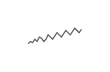
\begin{tikzpicture}[x=0.08em, y=0.08em, line width=0.4pt]
                \draw[FooterGray] (0,3) -- (1,4) -- (2,3.5) -- (3,5) -- (4,4) -- (5,6) -- (6,5.5) -- (7,4) -- (8,5) -- (9,7) -- (10,6) -- (11,5) -- (12,6.5) -- (13,8) -- (14,7) -- (15,6) -- (16,7.5) -- (17,9) -- (18,8) -- (19,7) -- (20,8.5) -- (21,10) -- (22,9) -- (23,8) -- (24,9.5);
            \end{tikzpicture}%
        }%
        \hskip0.5cm%
    }%
    \vskip6pt%
}

%=============================================================================
% PACKAGES
%=============================================================================
\usepackage[utf8]{inputenc}
\DeclareUnicodeCharacter{03B1}{\ensuremath{\alpha}}
\usepackage[T1]{fontenc}
\usepackage{amsmath, amssymb, amsthm}
\usepackage{mathtools}
\usepackage{bm}
\usepackage{tikz}
\usetikzlibrary{arrows.meta, positioning, shapes, calc, decorations.pathreplacing, shadings}
\usepackage{booktabs}
\usepackage{multirow}
\usepackage{array}
\usepackage{graphicx}
\usepackage{animate}
\usepackage{hyperref}
\usepackage{colortbl}
\usepackage{listings}
\lstset{language=Python, basicstyle=\ttfamily\scriptsize, keywordstyle=\color{MainBlue}\bfseries,
  commentstyle=\color{Forest}, stringstyle=\color{Crimson}, breaklines=true,
  frame=none, backgroundcolor=\color{VeryLightGray}, xleftmargin=2mm}
\hypersetup{colorlinks=true, linkcolor=MainBlue, urlcolor=MainBlue}
\graphicspath{{../../logos/}{../../charts/}{../../photos/}}
\usepackage{xcolor}
\hfuzz=2pt  % Suppress tiny overfull warnings (<2pt)
\vfuzz=2pt  % Suppress tiny vertical overfull warnings (<2pt)
% \mathrm in the sans-serif family of the slides (beamer resets \mathrm to the serif family at \begin{document};
% this hook runs after beamer's, so WN, Var, RMSE, ... in formulas match the surrounding text)
% Bold vectors and matrices in the same sans-serif family: \mathbf{A} in sans bold (beamer's own \mathbf came out in
% medium weight), and the bold upright Greek capitals of \boldsymbol / \bm (\bSigma, \bPhi, \boldsymbol{\Theta}) in
% cmss bold: bm.sty fixes its "boldoperators" font when it is loaded (serif cmbx), before beamer switches the
% operators to cmss, so it is reset here.
\AtBeginDocument{%
  \SetMathAlphabet{\mathrm}{normal}{\encodingdefault}{\sfdefault}{\mddefault}{n}%
  \SetMathAlphabet{\mathrm}{bold}{\encodingdefault}{\sfdefault}{bx}{n}%
  \SetMathAlphabet{\mathbf}{normal}{\encodingdefault}{\sfdefault}{bx}{n}%
  \SetMathAlphabet{\mathbf}{bold}{\encodingdefault}{\sfdefault}{bx}{n}%
  \SetSymbolFont{boldoperators}{normal}{OT1}{cmss}{bx}{n}%
  \SetSymbolFont{boldoperators}{bold}{OT1}{cmss}{bx}{n}}

%=============================================================================
% QUANTLET COMMANDS
%   \quantlet{<displayed name>}{<url>}       (generic, compatible with the older TSA decks)
%   \tsaquantlet{Ch_05}{TSA_ch5_garch}       -> https://github.com/danpele/Time-Series-Analysis/tree/main/Quantlets/Ch_05/TSA_ch5_garch
%   \qlurl{<folder>} is defined per chapter by the generator (Quantlets/Ch_NN/<folder>)
%=============================================================================
\newcommand{\tsarepo}{https://github.com/danpele/Time-Series-Analysis}
\newcommand{\tsaqlbase}{https://github.com/danpele/Time-Series-Analysis/tree/main/Quantlets}
\newcommand{\quantlet}[2]{%
    \hfill\href{#2}{%
        \raisebox{-0.15em}{
\includegraphics[height=0.7em]{ql_logo.png}}%
        \textcolor{MainBlue}{\tiny\ #1}%
    }%
}
\newcommand{\tsaquantlet}[2]{\quantlet{\detokenize{#2}}{\tsaqlbase/#1/#2}}

%=============================================================================
% NOTEBOOKS (Google Colab)
%   \colaburl{notebooks/EN/chapter5_seminar_notebook.ipynb} -> the Colab link of a file in the TSA repo
%   \nb: the chapter notebook (each seminar deck redefines it with \renewcommand)
%=============================================================================
\newcommand{\colaburl}[1]{https://colab.research.google.com/github/danpele/Time-Series-Analysis/blob/main/#1}
\newcommand{\nb}{https://colab.research.google.com/github/danpele/Time-Series-Analysis/tree/main/notebooks/EN}
\newcommand{\nbname}{notebooks/EN}

%=============================================================================
% SLIDE HELPERS (used by the generators; the same as in MFM)
%=============================================================================
% local font size for list bodies (the preamble forces \normalsize)
\newcommand{\itemsize}[1]{\setbeamertemplate{itemize/enumerate body begin}{#1}\setbeamertemplate{itemize/enumerate subbody begin}{#1}}
\newcommand{\intitle}[1]{{\hypersetup{urlcolor=white}#1}}   % white links inside coloured title bars
\newcommand{\imgcap}[1]{{\scriptsize #1}\\[0.5mm]}          % caption under a photo
\newcommand{\imgcredit}[2]{{\tiny\color{FooterGray}\href{#1}{#2}}}   % image credit: source URL, author/licence
\newcommand{\aiprompt}[1]{{\ttfamily\color{MainBlue}#1}}     % a prompt to an AI assistant

%=============================================================================
% SEMINARS: student version by default; the instructor wrapper *_solutions.tex sets \solutionstrue
%=============================================================================
\makeatletter\@ifundefined{ifsolutions}{\expandafter\newif\csname ifsolutions\endcsname}{}\makeatother
\newcommand{\solonly}[1]{\ifsolutions #1\fi}
\newcommand{\propsub}{\ifsolutions\else\framesubtitle{\ifdefined\tsalang Rezolvarea se discută la seminar\else Solution discussed in class\fi}\fi}

%=============================================================================
% APPENDIX AND CHAPTER LINKS (latex/appendix_links.py writes the calls; it also re-declares these
% macros before \begin{document}, so the decks compile with or without this preamble block)
%=============================================================================
\providecommand{\tsaapplink}[3]{\hypertarget{#2}{}\hyperlink{#1}{\beamergotobutton{#3}}}
\providecommand{\tsaappback}[2]{\begin{tikzpicture}[remember picture,overlay]\node[anchor=south east] at ([xshift=-3mm,yshift=7mm]current page.south east){\hyperlink{#1}{\beamerreturnbutton{#2}}};\end{tikzpicture}}
\providecommand{\tsachlink}[2]{\href{#1}{#2}}
\providecommand{\tsachlinkt}[2]{\href{#1}{\usebeamercolor[fg]{frametitle}#2}}

%=============================================================================
% QUANTINAR COMMAND: link către un curs Quantinar (subiecte avansate)
%=============================================================================
\newcommand{\quantinar}[2]{%
    \href{#2}{%
        \raisebox{-0.15em}{
\includegraphics[height=0.8em]{qr_logo.png}}%
        \textcolor{MainBlue}{\scriptsize\ #1}%
    }%
}

%=============================================================================
% CUSTOM TITLE PAGE
%=============================================================================
\defbeamertemplate*{title page}{hybrid}[1][]
{
    \vspace{0.2cm}
    % Logos row - top header (with clickable links)
    \begin{center}
        \href{https://www.ase.ro}{
\includegraphics[height=1.0cm]{ase_logo.png}}\hspace{0.3cm}%
        \href{https://theida.net}{
\includegraphics[height=1.0cm]{ida_logo.png}}\hspace{0.3cm}%
        \href{https://blockchain-research-center.com}{
\includegraphics[height=1.0cm]{brc_logo.png}}\hspace{0.3cm}%
        \href{https://www.ai4efin.ase.ro}{
\includegraphics[height=1.0cm]{ai4efin_logo.png}}\hspace{0.3cm}%
        \href{https://ipe.ro/new}{
\includegraphics[height=1.0cm]{acad_logo.png}}\hspace{0.3cm}%
        \href{https://www.digital-finance-msca.com}{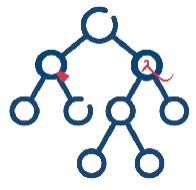
\includegraphics[height=1.0cm]{msca_logo.png}}%
    \end{center}

    \vspace{0.6cm}

    % Main title with Q logos on sides (with clickable links)
    \begin{center}
        \begin{minipage}{0.1\textwidth}
            \centering
            \href{https://quantlet.com}{
\includegraphics[height=1.1cm]{ql_logo.png}}
        \end{minipage}%
        \begin{minipage}{0.78\textwidth}
            \centering
            {\LARGE\bfseries\usebeamercolor[fg]{title}\inserttitle}

            \vspace{0.3cm}

            {\usebeamerfont{subtitle}\usebeamercolor[fg]{title}\insertsubtitle}
        \end{minipage}%
        \begin{minipage}{0.1\textwidth}
            \centering
            \href{https://quantinar.com}{
\includegraphics[height=1.1cm]{qr_logo.png}}
        \end{minipage}
    \end{center}

    \vspace{0.6cm}

    % Authors (left aligned)
    \hspace{0.5cm}{\usebeamerfont{author}\insertauthor}

    \vspace{0.3cm}

    % Institute/Affiliations (left aligned)
    \hspace{0.5cm}\begin{minipage}[t]{0.9\textwidth}
        \raggedright\small\insertinstitute
    \end{minipage}
}

%=============================================================================
% THEOREM ENVIRONMENTS
%=============================================================================
\theoremstyle{definition}
\setbeamertemplate{theorems}[numbered]
\ifdefined\tsalang
\newtheorem{defn}{Definiție}
\newtheorem{thm}{Teoremă}
\newtheorem{prop}{Propoziție}
\newtheorem{rmk}{Observație}
\else
\newtheorem{defn}{Definition}
\newtheorem{thm}{Theorem}
\newtheorem{prop}{Proposition}
\newtheorem{rmk}{Remark}
\fi

%=============================================================================
% CENTRED MINIPAGE (no extra vertical space)
%=============================================================================
\newenvironment{cminipage}[1]{%
    \par\noindent\hfill\begin{minipage}{#1}\ignorespaces
}{%
    \end{minipage}\hfill\null\par
}

%=============================================================================
% CUSTOM COMMANDS
%=============================================================================
\newcommand{\E}{\mathbb{E}}
\newcommand{\Var}{\text{Var}}
\newcommand{\Cov}{\text{Cov}}
\newcommand{\Corr}{\text{Corr}}
\newcommand{\R}{\mathbb{R}}
\newcommand{\N}{\mathbb{N}}
\newcommand{\Z}{\mathbb{Z}}
\newcommand{\B}{\mathbf{B}}
\newcommand{\imark}{\textcolor{MainBlue}{\textbullet}}
\newcommand{\RMSE}{\text{RMSE}}
\newcommand{\MAE}{\text{MAE}}
\newcommand{\MAPE}{\text{MAPE}}

% Boldface vector/matrix commands (VAR, VECM, state space; also used by the older TSA decks)
\newcommand{\bY}{\mathbf{Y}}
\newcommand{\bX}{\mathbf{X}}
\newcommand{\bA}{\mathbf{A}}
\newcommand{\bB}{\mathbf{B}}
\newcommand{\bepsilon}{\boldsymbol{\varepsilon}}
\newcommand{\bSigma}{\boldsymbol{\Sigma}}
\newcommand{\bPhi}{\boldsymbol{\Phi}}
\newcommand{\bGamma}{\boldsymbol{\Gamma}}
\newcommand{\bPi}{\boldsymbol{\Pi}}
\newcommand{\bc}{\mathbf{c}}
\newcommand{\balpha}{\boldsymbol{\alpha}}
\newcommand{\bbeta}{\boldsymbol{\beta}}
\newcommand{\bvarepsilon}{\boldsymbol{\varepsilon}}

% Legacy seminar marks (older TSA seminar decks)
\newcommand{\correct}{\textcolor{Forest}{\checkmark}}
\newcommand{\incorrect}{\textcolor{Crimson}{\texttimes}}
 se definește
%   \newcommand{\coursename}{Time Series Analysis}      (EN)
%   \newcommand{\coursename}{Serii de timp}       (RO)  și  \def\tsalang{ro}
% Fișierele .tex se află în EN/Courses, EN/Seminars, RO/Cursuri, RO/Seminarii (două niveluri sub rădăcină).
% Deck-urile sînt generate de latex/build_chapterN.py / build_seminarN.py (vezi latex/tsa_build.py).

\documentclass[9pt, aspectratio=169, t]{beamer}
\providecommand{\coursename}{Time Series Analysis}

% Ensure content fits on slides
\setbeamersize{text margin left=8mm, text margin right=8mm}
% Smaller institute font (title page)
\setbeamerfont{institute}{size=\footnotesize}

%=============================================================================
% THEME AND STYLE CONFIGURATION
%=============================================================================
\usetheme{default}
% Using default theme for clean header/footer control

% Color Palette (matching Redispatch PDF)
\definecolor{MainBlue}{RGB}{26, 58, 110}
\definecolor{AccentBlue}{RGB}{26, 58, 110}
\definecolor{IDAred}{RGB}{205, 0, 0}
\definecolor{DarkGray}{RGB}{51, 51, 51}
\definecolor{MediumGray}{RGB}{128, 128, 128}
\definecolor{LightGray}{RGB}{248, 248, 248}
\definecolor{VeryLightGray}{RGB}{235, 235, 235}
\definecolor{KeynoteGray}{RGB}{218, 218, 218}
\definecolor{SectionGray}{RGB}{120, 120, 120}
\definecolor{FooterGray}{RGB}{100, 100, 100}
\definecolor{Crimson}{RGB}{220, 53, 69}
\definecolor{Forest}{RGB}{46, 125, 50}
\definecolor{Amber}{RGB}{181, 133, 63}
\definecolor{Orange}{RGB}{230, 126, 34}
\definecolor{Purple}{RGB}{142, 68, 173}

% Gradient background (exact Keynote 315° gradient: white to RGB 218,218,218)
\setbeamertemplate{background}{%
    \begin{tikzpicture}[remember picture, overlay]
        \shade[shading=axis, shading angle=315,
        top color=white, bottom color=KeynoteGray]
        (current page.south west) rectangle (current page.north east);
    \end{tikzpicture}%
}
% Fallback solid color for compatibility
\setbeamercolor{background canvas}{bg=}

\setbeamercolor{palette primary}{bg=MainBlue, fg=white}
\setbeamercolor{palette secondary}{bg=MainBlue!85, fg=white}
\setbeamercolor{palette tertiary}{bg=MainBlue!70, fg=white}
\setbeamercolor{structure}{fg=MainBlue}
\setbeamercolor{title}{fg=IDAred}
\setbeamercolor{frametitle}{fg=IDAred, bg=}
\setbeamercolor{block title}{bg=MainBlue, fg=white}
\setbeamercolor{block body}{bg=VeryLightGray, fg=DarkGray}
\setbeamercolor{block title alerted}{bg=Crimson, fg=white}
\setbeamercolor{block body alerted}{bg=Crimson!8, fg=DarkGray}
\setbeamercolor{block title example}{bg=Forest, fg=white}
\setbeamercolor{block body example}{bg=Forest!8, fg=DarkGray}
\setbeamercolor{item}{fg=MainBlue}

% Footer colors (override Madrid theme blue)
\setbeamercolor{author in head/foot}{fg=FooterGray, bg=}
\setbeamercolor{title in head/foot}{fg=FooterGray, bg=}
\setbeamercolor{date in head/foot}{fg=FooterGray, bg=}
\setbeamercolor{section in head/foot}{fg=FooterGray, bg=}
\setbeamercolor{subsection in head/foot}{fg=FooterGray, bg=}

% Bullet styles (apply everywhere including blocks)
\setbeamertemplate{itemize item}{\color{MainBlue}$\boxdot$}
\setbeamertemplate{itemize subitem}{\color{MainBlue}$\blacktriangleright$}
\setbeamertemplate{itemize subsubitem}{\color{MainBlue}\tiny$\bullet$}
\setbeamertemplate{itemize/enumerate body begin}{\normalsize}
\setbeamertemplate{itemize/enumerate subbody begin}{\normalsize}

% Item spacing - compact style
\setlength{\leftmargini}{10pt}       % Level 1: minimal indent
\setlength{\leftmarginii}{10pt}      % Level 2: minimal additional indent
% Compact list spacing (zero extra space before/after lists in blocks)
\makeatletter
\def\@listi{\leftmargin\leftmargini \topsep 0pt \parsep 0pt \itemsep 0pt}
\def\@listii{\leftmargin\leftmarginii \topsep 0pt \parsep 0pt \itemsep 0pt}
\makeatother

\setbeamertemplate{navigation symbols}{}

%=============================================================================
% CUSTOM HEADLINE
%=============================================================================
\setbeamertemplate{headline}{%
    \vskip10pt%
    \hbox to \paperwidth{%
        \hskip0.5cm%
        {\small\color{FooterGray}\renewcommand{\hyperlink}[2]{##2}\insertsectionhead}%
        \hfill%
        \textcolor{FooterGray}{\small\insertframenumber}%
        \hskip0.5cm%
    }%
    \vskip4pt%
    {\color{FooterGray}\hrule height 0.4pt}%
}

%=============================================================================
% CUSTOM FOOTER
%=============================================================================
\usepackage{fontawesome5}

\setbeamertemplate{footline}{%
    {\color{FooterGray}\hrule height 0.4pt}%
    \vskip4pt%
    \hbox to \paperwidth{%
        \hskip0.5cm%
        \textcolor{FooterGray}{\small\coursename}%
        \hfill%
        \raisebox{-0.1em}{%
            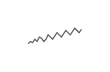
\begin{tikzpicture}[x=0.08em, y=0.08em, line width=0.4pt]
                \draw[FooterGray] (0,3) -- (1,4) -- (2,3.5) -- (3,5) -- (4,4) -- (5,6) -- (6,5.5) -- (7,4) -- (8,5) -- (9,7) -- (10,6) -- (11,5) -- (12,6.5) -- (13,8) -- (14,7) -- (15,6) -- (16,7.5) -- (17,9) -- (18,8) -- (19,7) -- (20,8.5) -- (21,10) -- (22,9) -- (23,8) -- (24,9.5);
            \end{tikzpicture}%
        }%
        \hskip0.5cm%
    }%
    \vskip6pt%
}

%=============================================================================
% PACKAGES
%=============================================================================
\usepackage[utf8]{inputenc}
\DeclareUnicodeCharacter{03B1}{\ensuremath{\alpha}}
\usepackage[T1]{fontenc}
\usepackage{amsmath, amssymb, amsthm}
\usepackage{mathtools}
\usepackage{bm}
\usepackage{tikz}
\usetikzlibrary{arrows.meta, positioning, shapes, calc, decorations.pathreplacing, shadings}
\usepackage{booktabs}
\usepackage{multirow}
\usepackage{array}
\usepackage{graphicx}
\usepackage{animate}
\usepackage{hyperref}
\usepackage{colortbl}
\usepackage{listings}
\lstset{language=Python, basicstyle=\ttfamily\scriptsize, keywordstyle=\color{MainBlue}\bfseries,
  commentstyle=\color{Forest}, stringstyle=\color{Crimson}, breaklines=true,
  frame=none, backgroundcolor=\color{VeryLightGray}, xleftmargin=2mm}
\hypersetup{colorlinks=true, linkcolor=MainBlue, urlcolor=MainBlue}
\graphicspath{{../../logos/}{../../charts/}{../../photos/}}
\usepackage{xcolor}
\hfuzz=2pt  % Suppress tiny overfull warnings (<2pt)
\vfuzz=2pt  % Suppress tiny vertical overfull warnings (<2pt)
% \mathrm in the sans-serif family of the slides (beamer resets \mathrm to the serif family at \begin{document};
% this hook runs after beamer's, so WN, Var, RMSE, ... in formulas match the surrounding text)
% Bold vectors and matrices in the same sans-serif family: \mathbf{A} in sans bold (beamer's own \mathbf came out in
% medium weight), and the bold upright Greek capitals of \boldsymbol / \bm (\bSigma, \bPhi, \boldsymbol{\Theta}) in
% cmss bold: bm.sty fixes its "boldoperators" font when it is loaded (serif cmbx), before beamer switches the
% operators to cmss, so it is reset here.
\AtBeginDocument{%
  \SetMathAlphabet{\mathrm}{normal}{\encodingdefault}{\sfdefault}{\mddefault}{n}%
  \SetMathAlphabet{\mathrm}{bold}{\encodingdefault}{\sfdefault}{bx}{n}%
  \SetMathAlphabet{\mathbf}{normal}{\encodingdefault}{\sfdefault}{bx}{n}%
  \SetMathAlphabet{\mathbf}{bold}{\encodingdefault}{\sfdefault}{bx}{n}%
  \SetSymbolFont{boldoperators}{normal}{OT1}{cmss}{bx}{n}%
  \SetSymbolFont{boldoperators}{bold}{OT1}{cmss}{bx}{n}}

%=============================================================================
% QUANTLET COMMANDS
%   \quantlet{<displayed name>}{<url>}       (generic, compatible with the older TSA decks)
%   \tsaquantlet{Ch_05}{TSA_ch5_garch}       -> https://github.com/danpele/Time-Series-Analysis/tree/main/Quantlets/Ch_05/TSA_ch5_garch
%   \qlurl{<folder>} is defined per chapter by the generator (Quantlets/Ch_NN/<folder>)
%=============================================================================
\newcommand{\tsarepo}{https://github.com/danpele/Time-Series-Analysis}
\newcommand{\tsaqlbase}{https://github.com/danpele/Time-Series-Analysis/tree/main/Quantlets}
\newcommand{\quantlet}[2]{%
    \hfill\href{#2}{%
        \raisebox{-0.15em}{
\includegraphics[height=0.7em]{ql_logo.png}}%
        \textcolor{MainBlue}{\tiny\ #1}%
    }%
}
\newcommand{\tsaquantlet}[2]{\quantlet{\detokenize{#2}}{\tsaqlbase/#1/#2}}

%=============================================================================
% NOTEBOOKS (Google Colab)
%   \colaburl{notebooks/EN/chapter5_seminar_notebook.ipynb} -> the Colab link of a file in the TSA repo
%   \nb: the chapter notebook (each seminar deck redefines it with \renewcommand)
%=============================================================================
\newcommand{\colaburl}[1]{https://colab.research.google.com/github/danpele/Time-Series-Analysis/blob/main/#1}
\newcommand{\nb}{https://colab.research.google.com/github/danpele/Time-Series-Analysis/tree/main/notebooks/EN}
\newcommand{\nbname}{notebooks/EN}

%=============================================================================
% SLIDE HELPERS (used by the generators; the same as in MFM)
%=============================================================================
% local font size for list bodies (the preamble forces \normalsize)
\newcommand{\itemsize}[1]{\setbeamertemplate{itemize/enumerate body begin}{#1}\setbeamertemplate{itemize/enumerate subbody begin}{#1}}
\newcommand{\intitle}[1]{{\hypersetup{urlcolor=white}#1}}   % white links inside coloured title bars
\newcommand{\imgcap}[1]{{\scriptsize #1}\\[0.5mm]}          % caption under a photo
\newcommand{\imgcredit}[2]{{\tiny\color{FooterGray}\href{#1}{#2}}}   % image credit: source URL, author/licence
\newcommand{\aiprompt}[1]{{\ttfamily\color{MainBlue}#1}}     % a prompt to an AI assistant

%=============================================================================
% SEMINARS: student version by default; the instructor wrapper *_solutions.tex sets \solutionstrue
%=============================================================================
\makeatletter\@ifundefined{ifsolutions}{\expandafter\newif\csname ifsolutions\endcsname}{}\makeatother
\newcommand{\solonly}[1]{\ifsolutions #1\fi}
\newcommand{\propsub}{\ifsolutions\else\framesubtitle{\ifdefined\tsalang Rezolvarea se discută la seminar\else Solution discussed in class\fi}\fi}

%=============================================================================
% APPENDIX AND CHAPTER LINKS (latex/appendix_links.py writes the calls; it also re-declares these
% macros before \begin{document}, so the decks compile with or without this preamble block)
%=============================================================================
\providecommand{\tsaapplink}[3]{\hypertarget{#2}{}\hyperlink{#1}{\beamergotobutton{#3}}}
\providecommand{\tsaappback}[2]{\begin{tikzpicture}[remember picture,overlay]\node[anchor=south east] at ([xshift=-3mm,yshift=7mm]current page.south east){\hyperlink{#1}{\beamerreturnbutton{#2}}};\end{tikzpicture}}
\providecommand{\tsachlink}[2]{\href{#1}{#2}}
\providecommand{\tsachlinkt}[2]{\href{#1}{\usebeamercolor[fg]{frametitle}#2}}

%=============================================================================
% QUANTINAR COMMAND: link către un curs Quantinar (subiecte avansate)
%=============================================================================
\newcommand{\quantinar}[2]{%
    \href{#2}{%
        \raisebox{-0.15em}{
\includegraphics[height=0.8em]{qr_logo.png}}%
        \textcolor{MainBlue}{\scriptsize\ #1}%
    }%
}

%=============================================================================
% CUSTOM TITLE PAGE
%=============================================================================
\defbeamertemplate*{title page}{hybrid}[1][]
{
    \vspace{0.2cm}
    % Logos row - top header (with clickable links)
    \begin{center}
        \href{https://www.ase.ro}{
\includegraphics[height=1.0cm]{ase_logo.png}}\hspace{0.3cm}%
        \href{https://theida.net}{
\includegraphics[height=1.0cm]{ida_logo.png}}\hspace{0.3cm}%
        \href{https://blockchain-research-center.com}{
\includegraphics[height=1.0cm]{brc_logo.png}}\hspace{0.3cm}%
        \href{https://www.ai4efin.ase.ro}{
\includegraphics[height=1.0cm]{ai4efin_logo.png}}\hspace{0.3cm}%
        \href{https://ipe.ro/new}{
\includegraphics[height=1.0cm]{acad_logo.png}}\hspace{0.3cm}%
        \href{https://www.digital-finance-msca.com}{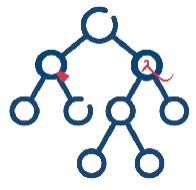
\includegraphics[height=1.0cm]{msca_logo.png}}%
    \end{center}

    \vspace{0.6cm}

    % Main title with Q logos on sides (with clickable links)
    \begin{center}
        \begin{minipage}{0.1\textwidth}
            \centering
            \href{https://quantlet.com}{
\includegraphics[height=1.1cm]{ql_logo.png}}
        \end{minipage}%
        \begin{minipage}{0.78\textwidth}
            \centering
            {\LARGE\bfseries\usebeamercolor[fg]{title}\inserttitle}

            \vspace{0.3cm}

            {\usebeamerfont{subtitle}\usebeamercolor[fg]{title}\insertsubtitle}
        \end{minipage}%
        \begin{minipage}{0.1\textwidth}
            \centering
            \href{https://quantinar.com}{
\includegraphics[height=1.1cm]{qr_logo.png}}
        \end{minipage}
    \end{center}

    \vspace{0.6cm}

    % Authors (left aligned)
    \hspace{0.5cm}{\usebeamerfont{author}\insertauthor}

    \vspace{0.3cm}

    % Institute/Affiliations (left aligned)
    \hspace{0.5cm}\begin{minipage}[t]{0.9\textwidth}
        \raggedright\small\insertinstitute
    \end{minipage}
}

%=============================================================================
% THEOREM ENVIRONMENTS
%=============================================================================
\theoremstyle{definition}
\setbeamertemplate{theorems}[numbered]
\ifdefined\tsalang
\newtheorem{defn}{Definiție}
\newtheorem{thm}{Teoremă}
\newtheorem{prop}{Propoziție}
\newtheorem{rmk}{Observație}
\else
\newtheorem{defn}{Definition}
\newtheorem{thm}{Theorem}
\newtheorem{prop}{Proposition}
\newtheorem{rmk}{Remark}
\fi

%=============================================================================
% CENTRED MINIPAGE (no extra vertical space)
%=============================================================================
\newenvironment{cminipage}[1]{%
    \par\noindent\hfill\begin{minipage}{#1}\ignorespaces
}{%
    \end{minipage}\hfill\null\par
}

%=============================================================================
% CUSTOM COMMANDS
%=============================================================================
\newcommand{\E}{\mathbb{E}}
\newcommand{\Var}{\text{Var}}
\newcommand{\Cov}{\text{Cov}}
\newcommand{\Corr}{\text{Corr}}
\newcommand{\R}{\mathbb{R}}
\newcommand{\N}{\mathbb{N}}
\newcommand{\Z}{\mathbb{Z}}
\newcommand{\B}{\mathbf{B}}
\newcommand{\imark}{\textcolor{MainBlue}{\textbullet}}
\newcommand{\RMSE}{\text{RMSE}}
\newcommand{\MAE}{\text{MAE}}
\newcommand{\MAPE}{\text{MAPE}}

% Boldface vector/matrix commands (VAR, VECM, state space; also used by the older TSA decks)
\newcommand{\bY}{\mathbf{Y}}
\newcommand{\bX}{\mathbf{X}}
\newcommand{\bA}{\mathbf{A}}
\newcommand{\bB}{\mathbf{B}}
\newcommand{\bepsilon}{\boldsymbol{\varepsilon}}
\newcommand{\bSigma}{\boldsymbol{\Sigma}}
\newcommand{\bPhi}{\boldsymbol{\Phi}}
\newcommand{\bGamma}{\boldsymbol{\Gamma}}
\newcommand{\bPi}{\boldsymbol{\Pi}}
\newcommand{\bc}{\mathbf{c}}
\newcommand{\balpha}{\boldsymbol{\alpha}}
\newcommand{\bbeta}{\boldsymbol{\beta}}
\newcommand{\bvarepsilon}{\boldsymbol{\varepsilon}}

% Legacy seminar marks (older TSA seminar decks)
\newcommand{\correct}{\textcolor{Forest}{\checkmark}}
\newcommand{\incorrect}{\textcolor{Crimson}{\texttimes}}
 se definește
%   \newcommand{\coursename}{Time Series Analysis}      (EN)
%   \newcommand{\coursename}{Serii de timp}       (RO)  și  \def\tsalang{ro}
% Fișierele .tex se află în EN/Courses, EN/Seminars, RO/Cursuri, RO/Seminarii (două niveluri sub rădăcină).
% Deck-urile sînt generate de latex/build_chapterN.py / build_seminarN.py (vezi latex/tsa_build.py).

\documentclass[9pt, aspectratio=169, t]{beamer}
\providecommand{\coursename}{Time Series Analysis}

% Ensure content fits on slides
\setbeamersize{text margin left=8mm, text margin right=8mm}
% Smaller institute font (title page)
\setbeamerfont{institute}{size=\footnotesize}

%=============================================================================
% THEME AND STYLE CONFIGURATION
%=============================================================================
\usetheme{default}
% Using default theme for clean header/footer control

% Color Palette (matching Redispatch PDF)
\definecolor{MainBlue}{RGB}{26, 58, 110}
\definecolor{AccentBlue}{RGB}{26, 58, 110}
\definecolor{IDAred}{RGB}{205, 0, 0}
\definecolor{DarkGray}{RGB}{51, 51, 51}
\definecolor{MediumGray}{RGB}{128, 128, 128}
\definecolor{LightGray}{RGB}{248, 248, 248}
\definecolor{VeryLightGray}{RGB}{235, 235, 235}
\definecolor{KeynoteGray}{RGB}{218, 218, 218}
\definecolor{SectionGray}{RGB}{120, 120, 120}
\definecolor{FooterGray}{RGB}{100, 100, 100}
\definecolor{Crimson}{RGB}{220, 53, 69}
\definecolor{Forest}{RGB}{46, 125, 50}
\definecolor{Amber}{RGB}{181, 133, 63}
\definecolor{Orange}{RGB}{230, 126, 34}
\definecolor{Purple}{RGB}{142, 68, 173}

% Gradient background (exact Keynote 315° gradient: white to RGB 218,218,218)
\setbeamertemplate{background}{%
    \begin{tikzpicture}[remember picture, overlay]
        \shade[shading=axis, shading angle=315,
        top color=white, bottom color=KeynoteGray]
        (current page.south west) rectangle (current page.north east);
    \end{tikzpicture}%
}
% Fallback solid color for compatibility
\setbeamercolor{background canvas}{bg=}

\setbeamercolor{palette primary}{bg=MainBlue, fg=white}
\setbeamercolor{palette secondary}{bg=MainBlue!85, fg=white}
\setbeamercolor{palette tertiary}{bg=MainBlue!70, fg=white}
\setbeamercolor{structure}{fg=MainBlue}
\setbeamercolor{title}{fg=IDAred}
\setbeamercolor{frametitle}{fg=IDAred, bg=}
\setbeamercolor{block title}{bg=MainBlue, fg=white}
\setbeamercolor{block body}{bg=VeryLightGray, fg=DarkGray}
\setbeamercolor{block title alerted}{bg=Crimson, fg=white}
\setbeamercolor{block body alerted}{bg=Crimson!8, fg=DarkGray}
\setbeamercolor{block title example}{bg=Forest, fg=white}
\setbeamercolor{block body example}{bg=Forest!8, fg=DarkGray}
\setbeamercolor{item}{fg=MainBlue}

% Footer colors (override Madrid theme blue)
\setbeamercolor{author in head/foot}{fg=FooterGray, bg=}
\setbeamercolor{title in head/foot}{fg=FooterGray, bg=}
\setbeamercolor{date in head/foot}{fg=FooterGray, bg=}
\setbeamercolor{section in head/foot}{fg=FooterGray, bg=}
\setbeamercolor{subsection in head/foot}{fg=FooterGray, bg=}

% Bullet styles (apply everywhere including blocks)
\setbeamertemplate{itemize item}{\color{MainBlue}$\boxdot$}
\setbeamertemplate{itemize subitem}{\color{MainBlue}$\blacktriangleright$}
\setbeamertemplate{itemize subsubitem}{\color{MainBlue}\tiny$\bullet$}
\setbeamertemplate{itemize/enumerate body begin}{\normalsize}
\setbeamertemplate{itemize/enumerate subbody begin}{\normalsize}

% Item spacing - compact style
\setlength{\leftmargini}{10pt}       % Level 1: minimal indent
\setlength{\leftmarginii}{10pt}      % Level 2: minimal additional indent
% Compact list spacing (zero extra space before/after lists in blocks)
\makeatletter
\def\@listi{\leftmargin\leftmargini \topsep 0pt \parsep 0pt \itemsep 0pt}
\def\@listii{\leftmargin\leftmarginii \topsep 0pt \parsep 0pt \itemsep 0pt}
\makeatother

\setbeamertemplate{navigation symbols}{}

%=============================================================================
% CUSTOM HEADLINE
%=============================================================================
\setbeamertemplate{headline}{%
    \vskip10pt%
    \hbox to \paperwidth{%
        \hskip0.5cm%
        {\small\color{FooterGray}\renewcommand{\hyperlink}[2]{##2}\insertsectionhead}%
        \hfill%
        \textcolor{FooterGray}{\small\insertframenumber}%
        \hskip0.5cm%
    }%
    \vskip4pt%
    {\color{FooterGray}\hrule height 0.4pt}%
}

%=============================================================================
% CUSTOM FOOTER
%=============================================================================
\usepackage{fontawesome5}

\setbeamertemplate{footline}{%
    {\color{FooterGray}\hrule height 0.4pt}%
    \vskip4pt%
    \hbox to \paperwidth{%
        \hskip0.5cm%
        \textcolor{FooterGray}{\small\coursename}%
        \hfill%
        \raisebox{-0.1em}{%
            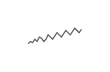
\begin{tikzpicture}[x=0.08em, y=0.08em, line width=0.4pt]
                \draw[FooterGray] (0,3) -- (1,4) -- (2,3.5) -- (3,5) -- (4,4) -- (5,6) -- (6,5.5) -- (7,4) -- (8,5) -- (9,7) -- (10,6) -- (11,5) -- (12,6.5) -- (13,8) -- (14,7) -- (15,6) -- (16,7.5) -- (17,9) -- (18,8) -- (19,7) -- (20,8.5) -- (21,10) -- (22,9) -- (23,8) -- (24,9.5);
            \end{tikzpicture}%
        }%
        \hskip0.5cm%
    }%
    \vskip6pt%
}

%=============================================================================
% PACKAGES
%=============================================================================
\usepackage[utf8]{inputenc}
\DeclareUnicodeCharacter{03B1}{\ensuremath{\alpha}}
\usepackage[T1]{fontenc}
\usepackage{amsmath, amssymb, amsthm}
\usepackage{mathtools}
\usepackage{bm}
\usepackage{tikz}
\usetikzlibrary{arrows.meta, positioning, shapes, calc, decorations.pathreplacing, shadings}
\usepackage{booktabs}
\usepackage{multirow}
\usepackage{array}
\usepackage{graphicx}
\usepackage{animate}
\usepackage{hyperref}
\usepackage{colortbl}
\usepackage{listings}
\lstset{language=Python, basicstyle=\ttfamily\scriptsize, keywordstyle=\color{MainBlue}\bfseries,
  commentstyle=\color{Forest}, stringstyle=\color{Crimson}, breaklines=true,
  frame=none, backgroundcolor=\color{VeryLightGray}, xleftmargin=2mm}
\hypersetup{colorlinks=true, linkcolor=MainBlue, urlcolor=MainBlue}
\graphicspath{{../../logos/}{../../charts/}{../../photos/}}
\usepackage{xcolor}
\hfuzz=2pt  % Suppress tiny overfull warnings (<2pt)
\vfuzz=2pt  % Suppress tiny vertical overfull warnings (<2pt)
% \mathrm in the sans-serif family of the slides (beamer resets \mathrm to the serif family at \begin{document};
% this hook runs after beamer's, so WN, Var, RMSE, ... in formulas match the surrounding text)
% Bold vectors and matrices in the same sans-serif family: \mathbf{A} in sans bold (beamer's own \mathbf came out in
% medium weight), and the bold upright Greek capitals of \boldsymbol / \bm (\bSigma, \bPhi, \boldsymbol{\Theta}) in
% cmss bold: bm.sty fixes its "boldoperators" font when it is loaded (serif cmbx), before beamer switches the
% operators to cmss, so it is reset here.
\AtBeginDocument{%
  \SetMathAlphabet{\mathrm}{normal}{\encodingdefault}{\sfdefault}{\mddefault}{n}%
  \SetMathAlphabet{\mathrm}{bold}{\encodingdefault}{\sfdefault}{bx}{n}%
  \SetMathAlphabet{\mathbf}{normal}{\encodingdefault}{\sfdefault}{bx}{n}%
  \SetMathAlphabet{\mathbf}{bold}{\encodingdefault}{\sfdefault}{bx}{n}%
  \SetSymbolFont{boldoperators}{normal}{OT1}{cmss}{bx}{n}%
  \SetSymbolFont{boldoperators}{bold}{OT1}{cmss}{bx}{n}}

%=============================================================================
% QUANTLET COMMANDS
%   \quantlet{<displayed name>}{<url>}       (generic, compatible with the older TSA decks)
%   \tsaquantlet{Ch_05}{TSA_ch5_garch}       -> https://github.com/danpele/Time-Series-Analysis/tree/main/Quantlets/Ch_05/TSA_ch5_garch
%   \qlurl{<folder>} is defined per chapter by the generator (Quantlets/Ch_NN/<folder>)
%=============================================================================
\newcommand{\tsarepo}{https://github.com/danpele/Time-Series-Analysis}
\newcommand{\tsaqlbase}{https://github.com/danpele/Time-Series-Analysis/tree/main/Quantlets}
\newcommand{\quantlet}[2]{%
    \hfill\href{#2}{%
        \raisebox{-0.15em}{
\includegraphics[height=0.7em]{ql_logo.png}}%
        \textcolor{MainBlue}{\tiny\ #1}%
    }%
}
\newcommand{\tsaquantlet}[2]{\quantlet{\detokenize{#2}}{\tsaqlbase/#1/#2}}

%=============================================================================
% NOTEBOOKS (Google Colab)
%   \colaburl{notebooks/EN/chapter5_seminar_notebook.ipynb} -> the Colab link of a file in the TSA repo
%   \nb: the chapter notebook (each seminar deck redefines it with \renewcommand)
%=============================================================================
\newcommand{\colaburl}[1]{https://colab.research.google.com/github/danpele/Time-Series-Analysis/blob/main/#1}
\newcommand{\nb}{https://colab.research.google.com/github/danpele/Time-Series-Analysis/tree/main/notebooks/EN}
\newcommand{\nbname}{notebooks/EN}

%=============================================================================
% SLIDE HELPERS (used by the generators; the same as in MFM)
%=============================================================================
% local font size for list bodies (the preamble forces \normalsize)
\newcommand{\itemsize}[1]{\setbeamertemplate{itemize/enumerate body begin}{#1}\setbeamertemplate{itemize/enumerate subbody begin}{#1}}
\newcommand{\intitle}[1]{{\hypersetup{urlcolor=white}#1}}   % white links inside coloured title bars
\newcommand{\imgcap}[1]{{\scriptsize #1}\\[0.5mm]}          % caption under a photo
\newcommand{\imgcredit}[2]{{\tiny\color{FooterGray}\href{#1}{#2}}}   % image credit: source URL, author/licence
\newcommand{\aiprompt}[1]{{\ttfamily\color{MainBlue}#1}}     % a prompt to an AI assistant

%=============================================================================
% SEMINARS: student version by default; the instructor wrapper *_solutions.tex sets \solutionstrue
%=============================================================================
\makeatletter\@ifundefined{ifsolutions}{\expandafter\newif\csname ifsolutions\endcsname}{}\makeatother
\newcommand{\solonly}[1]{\ifsolutions #1\fi}
\newcommand{\propsub}{\ifsolutions\else\framesubtitle{\ifdefined\tsalang Rezolvarea se discută la seminar\else Solution discussed in class\fi}\fi}

%=============================================================================
% APPENDIX AND CHAPTER LINKS (latex/appendix_links.py writes the calls; it also re-declares these
% macros before \begin{document}, so the decks compile with or without this preamble block)
%=============================================================================
\providecommand{\tsaapplink}[3]{\hypertarget{#2}{}\hyperlink{#1}{\beamergotobutton{#3}}}
\providecommand{\tsaappback}[2]{\begin{tikzpicture}[remember picture,overlay]\node[anchor=south east] at ([xshift=-3mm,yshift=7mm]current page.south east){\hyperlink{#1}{\beamerreturnbutton{#2}}};\end{tikzpicture}}
\providecommand{\tsachlink}[2]{\href{#1}{#2}}
\providecommand{\tsachlinkt}[2]{\href{#1}{\usebeamercolor[fg]{frametitle}#2}}

%=============================================================================
% QUANTINAR COMMAND: link către un curs Quantinar (subiecte avansate)
%=============================================================================
\newcommand{\quantinar}[2]{%
    \href{#2}{%
        \raisebox{-0.15em}{
\includegraphics[height=0.8em]{qr_logo.png}}%
        \textcolor{MainBlue}{\scriptsize\ #1}%
    }%
}

%=============================================================================
% CUSTOM TITLE PAGE
%=============================================================================
\defbeamertemplate*{title page}{hybrid}[1][]
{
    \vspace{0.2cm}
    % Logos row - top header (with clickable links)
    \begin{center}
        \href{https://www.ase.ro}{
\includegraphics[height=1.0cm]{ase_logo.png}}\hspace{0.3cm}%
        \href{https://theida.net}{
\includegraphics[height=1.0cm]{ida_logo.png}}\hspace{0.3cm}%
        \href{https://blockchain-research-center.com}{
\includegraphics[height=1.0cm]{brc_logo.png}}\hspace{0.3cm}%
        \href{https://www.ai4efin.ase.ro}{
\includegraphics[height=1.0cm]{ai4efin_logo.png}}\hspace{0.3cm}%
        \href{https://ipe.ro/new}{
\includegraphics[height=1.0cm]{acad_logo.png}}\hspace{0.3cm}%
        \href{https://www.digital-finance-msca.com}{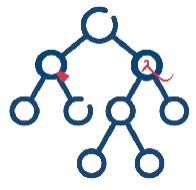
\includegraphics[height=1.0cm]{msca_logo.png}}%
    \end{center}

    \vspace{0.6cm}

    % Main title with Q logos on sides (with clickable links)
    \begin{center}
        \begin{minipage}{0.1\textwidth}
            \centering
            \href{https://quantlet.com}{
\includegraphics[height=1.1cm]{ql_logo.png}}
        \end{minipage}%
        \begin{minipage}{0.78\textwidth}
            \centering
            {\LARGE\bfseries\usebeamercolor[fg]{title}\inserttitle}

            \vspace{0.3cm}

            {\usebeamerfont{subtitle}\usebeamercolor[fg]{title}\insertsubtitle}
        \end{minipage}%
        \begin{minipage}{0.1\textwidth}
            \centering
            \href{https://quantinar.com}{
\includegraphics[height=1.1cm]{qr_logo.png}}
        \end{minipage}
    \end{center}

    \vspace{0.6cm}

    % Authors (left aligned)
    \hspace{0.5cm}{\usebeamerfont{author}\insertauthor}

    \vspace{0.3cm}

    % Institute/Affiliations (left aligned)
    \hspace{0.5cm}\begin{minipage}[t]{0.9\textwidth}
        \raggedright\small\insertinstitute
    \end{minipage}
}

%=============================================================================
% THEOREM ENVIRONMENTS
%=============================================================================
\theoremstyle{definition}
\setbeamertemplate{theorems}[numbered]
\ifdefined\tsalang
\newtheorem{defn}{Definiție}
\newtheorem{thm}{Teoremă}
\newtheorem{prop}{Propoziție}
\newtheorem{rmk}{Observație}
\else
\newtheorem{defn}{Definition}
\newtheorem{thm}{Theorem}
\newtheorem{prop}{Proposition}
\newtheorem{rmk}{Remark}
\fi

%=============================================================================
% CENTRED MINIPAGE (no extra vertical space)
%=============================================================================
\newenvironment{cminipage}[1]{%
    \par\noindent\hfill\begin{minipage}{#1}\ignorespaces
}{%
    \end{minipage}\hfill\null\par
}

%=============================================================================
% CUSTOM COMMANDS
%=============================================================================
\newcommand{\E}{\mathbb{E}}
\newcommand{\Var}{\text{Var}}
\newcommand{\Cov}{\text{Cov}}
\newcommand{\Corr}{\text{Corr}}
\newcommand{\R}{\mathbb{R}}
\newcommand{\N}{\mathbb{N}}
\newcommand{\Z}{\mathbb{Z}}
\newcommand{\B}{\mathbf{B}}
\newcommand{\imark}{\textcolor{MainBlue}{\textbullet}}
\newcommand{\RMSE}{\text{RMSE}}
\newcommand{\MAE}{\text{MAE}}
\newcommand{\MAPE}{\text{MAPE}}

% Boldface vector/matrix commands (VAR, VECM, state space; also used by the older TSA decks)
\newcommand{\bY}{\mathbf{Y}}
\newcommand{\bX}{\mathbf{X}}
\newcommand{\bA}{\mathbf{A}}
\newcommand{\bB}{\mathbf{B}}
\newcommand{\bepsilon}{\boldsymbol{\varepsilon}}
\newcommand{\bSigma}{\boldsymbol{\Sigma}}
\newcommand{\bPhi}{\boldsymbol{\Phi}}
\newcommand{\bGamma}{\boldsymbol{\Gamma}}
\newcommand{\bPi}{\boldsymbol{\Pi}}
\newcommand{\bc}{\mathbf{c}}
\newcommand{\balpha}{\boldsymbol{\alpha}}
\newcommand{\bbeta}{\boldsymbol{\beta}}
\newcommand{\bvarepsilon}{\boldsymbol{\varepsilon}}

% Legacy seminar marks (older TSA seminar decks)
\newcommand{\correct}{\textcolor{Forest}{\checkmark}}
\newcommand{\incorrect}{\textcolor{Crimson}{\texttimes}}


\newcommand{\qlurl}[1]{https://github.com/danpele/Time-Series-Analysis/tree/main/Quantlets/Ch_01/#1}

% Clickable citations (DOIs verified via Crossref)
\newcommand{\refHP}{\href{https://doi.org/10.1007/978-3-031-13584-2}{Huang and Petukhina (2022)}}
\newcommand{\refFPP}{\href{https://otexts.com/fpp3/}{Hyndman and Athanasopoulos (2021)}}
\newcommand{\refBD}{\href{https://doi.org/10.1007/978-3-319-29854-2}{Brockwell and Davis (2016)}}
\newcommand{\refBDtm}{\href{https://doi.org/10.1007/978-1-4419-0320-4}{Brockwell and Davis (1991)}}
\newcommand{\refHamilton}{\href{https://doi.org/10.2307/j.ctv14jx6sm}{Hamilton (1994)}}
\newcommand{\refSS}{\href{https://doi.org/10.1007/978-3-319-52452-8}{Shumway and Stoffer (2017)}}
\newcommand{\refBP}{\href{https://doi.org/10.1080/01621459.1970.10481180}{Box and Pierce (1970)}}
\newcommand{\refLB}{\href{https://doi.org/10.1093/biomet/65.2.297}{Ljung and Box (1978)}}
\newcommand{\refBC}{\href{https://doi.org/10.1111/j.2517-6161.1964.tb00553.x}{Box and Cox (1964)}}
\newcommand{\refBartlett}{\href{https://doi.org/10.2307/2983611}{Bartlett (1946)}}
\newcommand{\refYule}{\href{https://doi.org/10.1098/rsta.1927.0007}{Yule (1927)}}
\newcommand{\refSlutzky}{\href{https://doi.org/10.2307/1907241}{Slutzky (1937)}}
\newcommand{\refGuerrero}{\href{https://doi.org/10.1002/for.3980120104}{Guerrero (1993)}}
\newcommand{\refKhinchin}{\href{https://doi.org/10.1007/BF01449156}{Khintchine (1934)}}
\newcommand{\refWold}{\href{https://archive.org/details/in.ernet.dli.2015.262214}{Wold (1938)}}
\newcommand{\refCobb}{\href{https://doi.org/10.1093/biomet/65.2.243}{Cobb (1978)}}

\title[Time Series Analysis]{Time Series Analysis}
\subtitle{Chapter 1: Stochastic processes and stationarity}
\author[D.T. Pele]{Daniel Traian PELE}
\institute{Bucharest University of Economic Studies\\
IDA Institute Digital Assets\\
Blockchain Research Center\\
AI4EFin Artificial Intelligence for Energy Finance\\
Romanian Academy, Institute for Economic Forecasting\\
MSCA Digital Finance}
\date{}

%=============================================================================
\providecommand{\tsaapplink}[3]{\hypertarget{#2}{}\hyperlink{#1}{\beamergotobutton{#3}}}  % APPLINKS-MACROS
\providecommand{\tsaappback}[2]{\begin{tikzpicture}[remember picture,overlay]\node[anchor=south east] at ([xshift=-3mm,yshift=7mm]current page.south east){\hyperlink{#1}{\beamerreturnbutton{#2}}};\end{tikzpicture}}  % APPLINKS-MACROS
\providecommand{\tsachlink}[2]{\href{#1}{#2}}  % APPLINKS-MACROS
\providecommand{\tsachlinkt}[2]{\href{#1}{\usebeamercolor[fg]{frametitle}#2}}  % APPLINKS-MACROS
\begin{document}
%=============================================================================

{
\setbeamertemplate{headline}{}
\setbeamertemplate{footline}{}
\begin{frame}[noframenumbering]
    \titlepage
\end{frame}
}
% BEGIN-ACRONYMS (generat de latex/acronyms.py; nu editati manual)
\begin{frame}{Acronyms used in this material}
\setbeamertemplate{itemize/enumerate body begin}{\footnotesize}
\begin{columns}[T]
\begin{column}{0.49\textwidth}
\begin{itemize}\setlength{\itemsep}{0pt}
    \item \textbf{ACF}: Autocorrelation Function
    \item \textbf{AI}: Artificial Intelligence
    \item \textbf{AR}: AutoRegressive (model)
    \item \textbf{ARIMA}: AutoRegressive Integrated Moving Average (model)
    \item \textbf{ARMA}: AutoRegressive Moving Average (model)
    \item \textbf{BET}: Bucharest Exchange Trading (index)
    \item \textbf{BNR}: Banca Națională a României (the National Bank of Romania)
    \item \textbf{BVB}: Bursa de Valori București (the Bucharest Stock Exchange)
\end{itemize}
\end{column}
\begin{column}{0.49\textwidth}
\begin{itemize}\setlength{\itemsep}{0pt}
    \item \textbf{EU}: European Union
    \item \textbf{GARCH}: Generalised AutoRegressive Conditional Heteroskedasticity
    \item \textbf{GDP}: Gross Domestic Product
    \item \textbf{HICP}: Harmonised Index of Consumer Prices
    \item \textbf{MA}: Moving Average
    \item \textbf{PACF}: Partial AutoCorrelation Function
    \item \textbf{SARIMA}: Seasonal ARIMA (model)
    \item \textbf{VAR}: Vector AutoRegression
\end{itemize}
\end{column}
\end{columns}
\end{frame}
% END-ACRONYMS

\begin{frame}{Today's question and route}
\itemsize{\small}
\begin{itemize}
    \item \textbf{Question}: we observe one path of a series, a single history; what can we learn from it about the mechanism that produced it?
    \begin{itemize}
        \item the answer rests on two assumptions: \textbf{stationarity} and \textbf{ergodicity}
        \item the main tool: the \textbf{autocorrelation function} (ACF)
    \end{itemize}
    \item \textbf{Route} of the chapter
    \begin{itemize}
        \item stochastic processes and their moments; strict and weak stationarity
        \item white noise and the random walk; the lag operator, differencing, the Wold decomposition, ergodicity
        \item sample ACF and PACF with confidence bands; the Box--Pierce and Ljung--Box tests
        \item transformations (log, differencing, Box--Cox) and a first look at real series
    \end{itemize}
    \item Seminar 1 comes before this lecture: its primer gives the definitions; here we derive and explain them
\end{itemize}
\end{frame}

\begin{frame}{Learning outcomes}
\itemsize{\small}
\begin{itemize}
    \item Define a stochastic process and its mean, autocovariance and autocorrelation functions
    \item Distinguish strict from weak stationarity, and check weak stationarity for simple processes
    \item Derive the moments of white noise, of a moving average and of a random walk
    \item Compute and read the sample ACF and PACF with their $\pm 1.96/\sqrt{T}$ bands
    \item Test for autocorrelation with the Box--Pierce and Ljung--Box statistics
    \item Choose a transformation (log, difference, Box--Cox) that makes a real series closer to stationary
\end{itemize}
\end{frame}

\begin{frame}{Reading and tools}
\itemsize{\small}
\begin{itemize}
    \item Textbook: \refHP, Ch.~1--2 (concepts, exploratory analysis)
    \begin{itemize}
        \item companion, free online: \refFPP, Ch.~2 (time series graphics) and Ch.~3 (transformations)
    \end{itemize}
    \item Theory: \refBD, Ch.~1; \refHamilton, Ch.~3
    \item Python Quantlets of this chapter: \href{https://github.com/danpele/Time-Series-Analysis/tree/main/Quantlets/Ch_01}{Quantlets/Ch\_01}
    \begin{itemize}
        \item ACF, PACF and portmanteau tests with \texttt{statsmodels}
    \end{itemize}
    \item Lecture notebook: \href{\colaburl{notebooks/EN/chapter1_lecture_notebook.ipynb}}{open in Google Colab}
    \item Video course: \quantinar{Applied Time Series Analysis with Python}{https://quantinar.com/course/137/applied-time-series-analysis-with-python}
\end{itemize}
\end{frame}


%=============================================================================
\section{Time series and stochastic processes}
%=============================================================================

\begin{frame}{Four series of this course}
\itemsize{\footnotesize}
\begin{center}
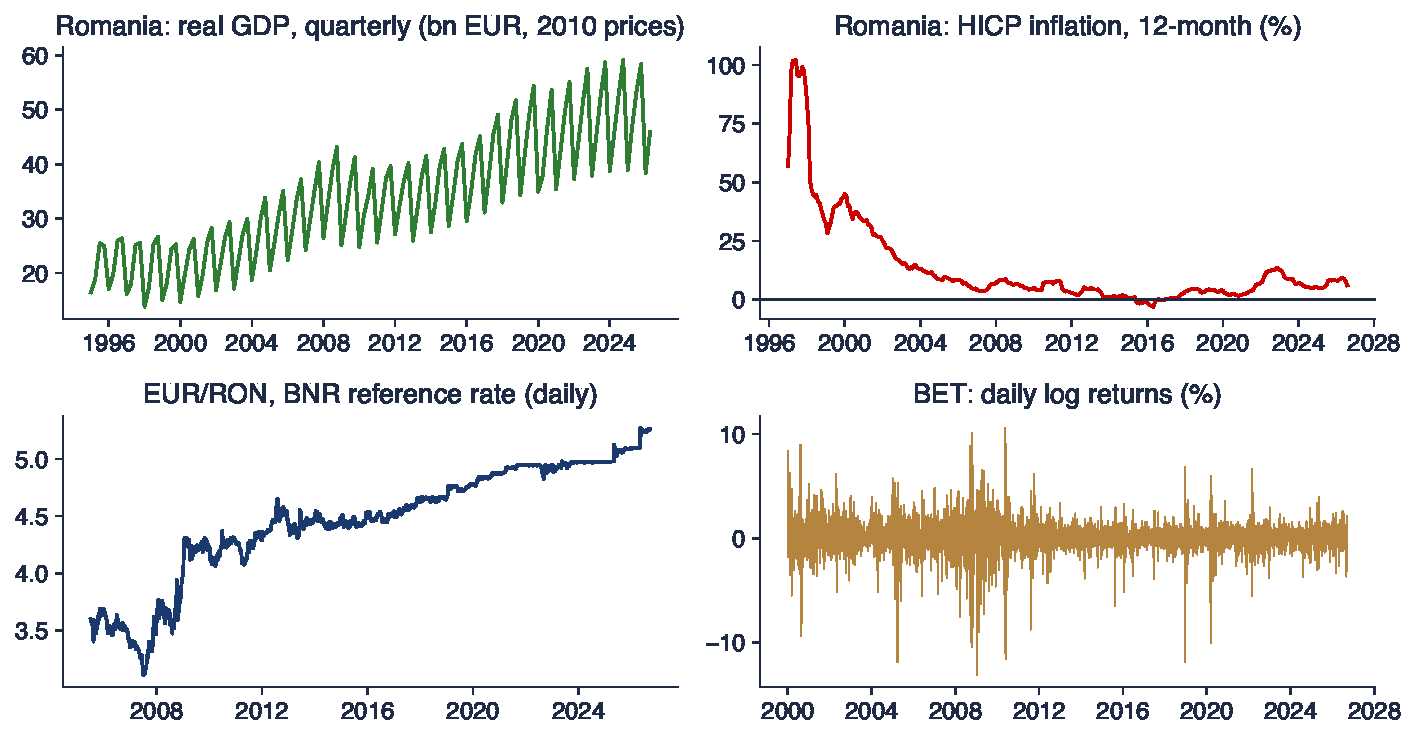
\includegraphics[width=0.97\textwidth,height=0.66\textheight,keepaspectratio]{tsa_ch1_four_series.pdf}
\end{center}
\vspace{-0.25cm}
\begin{itemize}
    \item Romanian real GDP, 1995Q1--2026Q2 (Eurostat); HICP inflation (Eurostat); EUR/RON, the BNR reference rate; BET daily log returns since 2000
    \item Four frequencies (quarterly, monthly, daily) and four kinds of behaviour
\end{itemize}
\quantlet{TSA\_ch1\_real\_series}{\qlurl{TSA_ch1_real_series}}
\end{frame}

\begin{frame}{Interpreting the four series}
\itemsize{\small}
\begin{itemize}
    \item \textbf{GDP}: from 16.5 to 45.9 bn EUR per quarter; a trend and a seasonal pattern whose swing grows with the level
    \begin{itemize}
        \item the mean of the series changes with time
    \end{itemize}
    \item \textbf{Inflation}: 102\% in June 1997, \ensuremath{-}3.0\% in May 2016, 6.1\% in August 2026
    \begin{itemize}
        \item a slow, persistent movement: this month resembles the previous one
    \end{itemize}
    \item \textbf{EUR/RON}: from 3.60 to 5.26 lei; it wanders without returning to a fixed level
    \begin{itemize}
        \item a candidate for a random walk (Section 3)
    \end{itemize}
    \item \textbf{BET returns}: they oscillate around a constant level close to 0; the extremes: $\ensuremath{-}13.1\%$ on 7 January 2009, $+10.6\%$ on 10 May 2010
    \begin{itemize}
        \item but the amplitude changes: standard deviation 3.62\% in September 2008--March 2009, 0.66\% in 2017
    \end{itemize}
\end{itemize}
\end{frame}

\begin{frame}{A time series as one realisation}
\itemsize{\small}
\begin{itemize}
    \item \textbf{Time series}: observations $x_1, x_2, \dots, x_T$ ordered in time, at equal intervals
    \begin{itemize}
        \item $T$ = sample size; $t$ = time index (day, month, quarter)
    \end{itemize}
    \item The key idea: each $x_t$ is the observed value of a \textbf{random variable} $X_t$
    \begin{itemize}
        \item the BET return of tomorrow is unknown today: it has a distribution of possible values
        \item history ran only once: we see one value from each distribution
    \end{itemize}
    \item Consequence: we need assumptions that link the distributions at different dates
    \begin{itemize}
        \item otherwise $T$ observations would estimate $T$ different means
    \end{itemize}
\end{itemize}
\end{frame}

\begin{frame}{Stochastic process}
\itemsize{\small}
\begin{itemize}
    \item \textbf{Definition}: a \textbf{stochastic process} is a family of random variables $\{X_t : t \in \mathcal{T}\}$ defined on the same probability space $(\Omega, \mathcal{F}, P)$
    \begin{itemize}
        \item $\mathcal{T} = \mathbb{Z}$ or $\{1, \dots, T\}$: \textbf{discrete time}, the case of this course
        \item $\Omega$: the set of possible ``histories'' $\omega$; $P$: their probabilities
    \end{itemize}
    \item Two ways to look at $X_t(\omega)$
    \begin{itemize}
        \item fix $t$: $X_t$ is a random variable (all values possible at date $t$)
        \item fix $\omega$: $t \mapsto X_t(\omega)$ is a \textbf{path} (trajectory, realisation): what we observe
    \end{itemize}
    \item The process is described by its \textbf{finite-dimensional distributions}: the joint distribution of $(X_{t_1}, \dots, X_{t_k})$ for any dates $t_1, \dots, t_k$
\end{itemize}
\end{frame}

\begin{frame}{An ensemble of paths}
\itemsize{\footnotesize}
\begin{center}
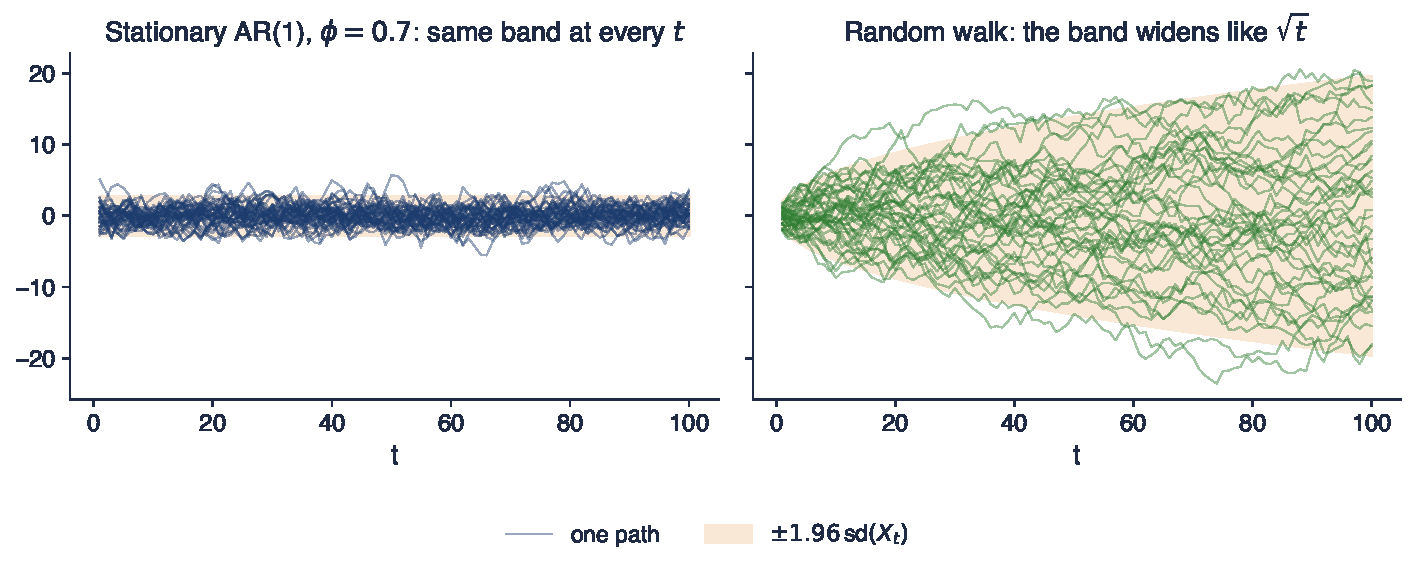
\includegraphics[width=0.97\textwidth,height=0.64\textheight,keepaspectratio]{tsa_ch1_ensemble.pdf}
\end{center}
\vspace{-0.25cm}
\begin{itemize}
    \item Left: 40 paths of $X_t = 0.7X_{t-1} + \varepsilon_t$, $\varepsilon_t \sim N(0, 1)$ i.i.d. (independent and identically distributed); right: 40 paths of $X_t = X_{t-1} + \varepsilon_t$, $X_0 = 0$
    \item The shaded band: $\pm 1.96$ standard deviations of $X_t$ at each $t$
\end{itemize}
\quantlet{TSA\_ch1\_processes}{\qlurl{TSA_ch1_processes}}
\end{frame}

\begin{frame}{Interpreting the ensemble}
\itemsize{\small}
\begin{itemize}
    \item A vertical slice at date $t$ shows the \textbf{distribution of $X_t$}; one path shows \textbf{one history}
    \begin{itemize}
        \item the moments of the process (mean, variance) are averages across paths, at a fixed $t$
    \end{itemize}
    \item Left: the same band at every $t$: $\mathrm{Var}(X_t) = 1/(1 - 0.7^2) = 1.96$, band $\pm 2.74$
    \begin{itemize}
        \item the distribution of $X_t$ does not depend on $t$: a first picture of \textbf{stationarity}
    \end{itemize}
    \item Right: the band widens; across 5000 simulated paths, $\mathrm{Var}(X_{100}) = 100.8$ (theory: 100)
    \begin{itemize}
        \item the distribution changes with $t$: the random walk is \textbf{not stationary}
    \end{itemize}
\end{itemize}
\end{frame}

\begin{frame}{Mean, autocovariance and autocorrelation functions}
\itemsize{\small}
\begin{itemize}
    \item For a process with $E[X_t^2] < \infty$ for every $t$:
    \begin{itemize}
        \item \textbf{mean function}: $\mu_t = E[X_t]$
        \item \textbf{autocovariance function}: $\gamma(t, s) = \mathrm{Cov}(X_t, X_s) = E[(X_t - \mu_t)(X_s - \mu_s)]$
        \item \textbf{autocorrelation function}: $\rho(t, s) = \gamma(t, s)/\sqrt{\gamma(t, t)\,\gamma(s, s)}$
    \end{itemize}
    \item ``Auto'': the covariance of the series with itself at two dates
    \begin{itemize}
        \item $\gamma(t, t) = \mathrm{Var}(X_t)$; $\rho(t, t) = 1$; $|\rho(t, s)| \le 1$ (Cauchy--Schwarz inequality)
    \end{itemize}
    \item \textbf{Example}: $X_t = a + bt + \varepsilon_t$, $\varepsilon_t$ i.i.d. with mean 0 and variance $\sigma^2$
    \begin{itemize}
        \item $\mu_t = a + bt$ depends on $t$; $\gamma(t, t) = \sigma^2$, $\gamma(t, s) = 0$ for $t \ne s$
    \end{itemize}
\end{itemize}
\end{frame}

\begin{frame}{Recap: Time series and stochastic processes}
\itemsize{\small}
\begin{itemize}
    \item A time series is one path of a stochastic process $\{X_t\}$
    \item Moments are averages across paths at fixed dates: $\mu_t$, $\gamma(t, s)$, $\rho(t, s)$
    \item With one path, we must assume these functions do not change with time
\end{itemize}
\end{frame}


%=============================================================================
\section{Stationarity}
%=============================================================================

\begin{frame}{Strict stationarity}
\itemsize{\small}
\begin{itemize}
    \item \textbf{Definition}: $\{X_t\}$ is \textbf{strictly stationary} if, for every $k \ge 1$, all dates $t_1, \dots, t_k$ and every shift $h$:
    \begin{itemize}
        \item $(X_{t_1}, \dots, X_{t_k}) \overset{d}{=} (X_{t_1 + h}, \dots, X_{t_k + h})$, where $\overset{d}{=}$ means equal joint distributions
    \end{itemize}
    \item Consequences
    \begin{itemize}
        \item $k = 1$: all $X_t$ have the same distribution
        \item $k = 2$: the joint distribution of $(X_t, X_{t+h})$ depends only on the lag $h$
    \end{itemize}
    \item Example: an i.i.d. sequence is strictly stationary
    \begin{itemize}
        \item the definition concerns entire distributions; the moments need not even exist (an i.i.d. Cauchy sequence)
    \end{itemize}
    \item Hard to check from data: we would need all joint distributions
\end{itemize}
\end{frame}

\begin{frame}{Weak stationarity}
\itemsize{\small}
\begin{itemize}
    \item \textbf{Definition} \refKhinchin: $\{X_t\}$ is \textbf{weakly stationary} (covariance stationary, second-order stationary) if
    \begin{itemize}
        \item (i) $E[X_t^2] < \infty$ for every $t$
        \item (ii) $E[X_t] = \mu$, the same for every $t$
        \item (iii) $\mathrm{Cov}(X_t, X_{t+h}) = \gamma(h)$ depends only on the lag $h$, not on $t$
    \end{itemize}
    \item Then the functions have one argument, the \textbf{lag} $h$:
    \begin{itemize}
        \item $\gamma(h) = \mathrm{Cov}(X_t, X_{t+h})$, $\gamma(0) = \mathrm{Var}(X_t)$
        \item $\rho(h) = \gamma(h)/\gamma(0)$: the \textbf{ACF} (autocorrelation function)
    \end{itemize}
    \item In this course, ``stationary'' means weakly stationary unless stated otherwise
\end{itemize}
\end{frame}

\begin{frame}{Strict and weak stationarity compared}
\itemsize{\small}
\begin{itemize}
    \item \textbf{Strict + finite variance $\Rightarrow$ weak}
    \begin{itemize}
        \item equal distributions give equal means; equal joint distributions of $(X_t, X_{t+h})$ give equal covariances
    \end{itemize}
    \item \textbf{Weak $\not\Rightarrow$ strict}
    \begin{itemize}
        \item weak stationarity fixes only the first two moments; the shape of the distribution may change (next slide)
    \end{itemize}
    \item \textbf{Strict $\not\Rightarrow$ weak} if the variance is infinite
    \begin{itemize}
        \item i.i.d. Student-t with 2 degrees of freedom: strictly stationary, no finite variance
    \end{itemize}
    \item \textbf{Gaussian processes}: all finite-dimensional distributions are multivariate Normal
    \begin{itemize}
        \item a Normal distribution is fixed by its means and covariances, so for them weak $\Leftrightarrow$ strict
    \end{itemize}
\end{itemize}
\end{frame}

\begin{frame}{Weakly but not strictly stationary}
\itemsize{\footnotesize}
\begin{center}
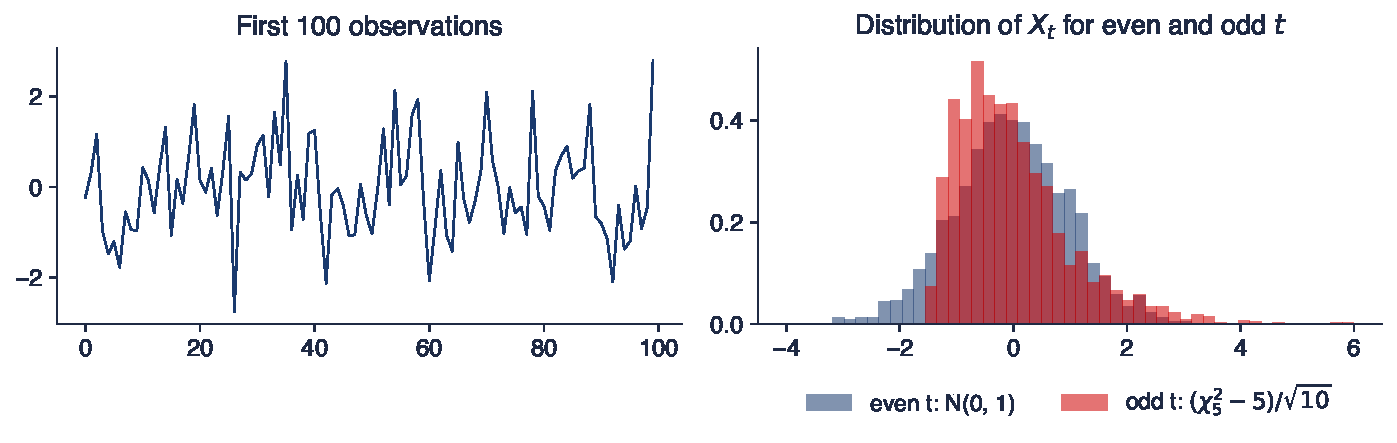
\includegraphics[width=0.97\textwidth,height=0.60\textheight,keepaspectratio]{tsa_ch1_counterexample.pdf}
\end{center}
\vspace{-0.25cm}
\begin{itemize}
    \item Independent $X_t$: $N(0, 1)$ for even $t$, $(\chi^2_5 - 5)/\sqrt{10}$ for odd $t$; both have mean 0 and variance 1
    \item Sample of 4000: variance 0.99 (even) and 1.00 (odd); skewness $\ensuremath{-}0.02$ and $1.30$ (theory: 0 and 1.26)
\end{itemize}
\quantlet{TSA\_ch1\_processes}{\qlurl{TSA_ch1_processes}}
\end{frame}

\begin{frame}{Interpreting the counterexample}
\itemsize{\small}
\begin{itemize}
    \item Weakly stationary: $E[X_t] = 0$, $\gamma(0) = 1$, $\gamma(h) = 0$ for $h \ne 0$, at every $t$
    \begin{itemize}
        \item the ACF cannot tell this process from Gaussian white noise
    \end{itemize}
    \item Not strictly stationary: the distribution of $X_t$ alternates between symmetric and right-skewed
    \begin{itemize}
        \item $P(X_t < -1.6)$: about 5\% for even $t$, 0 for odd $t$ ($X_t \ge -5/\sqrt{10} = -1.58$)
    \end{itemize}
    \item Lesson: second moments summarise dependence, but not the whole distribution; tail risk needs more (\tsachlink{https://danpele.github.io/Time-Series-Analysis/EN/Courses/chapter5_conditional_volatility_garch.pdf}{Chapter 5})
\end{itemize}
\end{frame}

\begin{frame}{Properties of the autocovariance function}
\itemsize{\small}
\begin{itemize}
    \item For a weakly stationary process:
    \begin{itemize}
        \item \textbf{symmetry}: $\gamma(-h) = \gamma(h)$, since $\mathrm{Cov}(X_t, X_{t-h}) = \mathrm{Cov}(X_{t-h}, X_t)$
        \item \textbf{bound}: $|\gamma(h)| \le \gamma(0)$, so $|\rho(h)| \le 1$
        \item \textbf{non-negative definiteness}: $\sum_{i,j} a_i a_j \gamma(i - j) \ge 0$ for all real $a_1, \dots, a_n$
    \end{itemize}
    \item Proof of the third property
    \begin{itemize}
        \item $0 \le \mathrm{Var}\big(\sum_i a_i X_i\big) = \sum_{i,j} a_i a_j \mathrm{Cov}(X_i, X_j) = \sum_{i,j} a_i a_j \gamma(i - j)$
    \end{itemize}
    \item Consequence: not every sequence is an ACF
    \begin{itemize}
        \item $\rho(1) = 0.9$, $\rho(2) = -0.9$ is impossible: with $a = (1, -1, -1)$, $\mathrm{Var}(X_1 - X_2 - X_3) = \gamma(0)(3 - 2\rho(1) - 2\rho(1) + 2\rho(2)) < 0$
    \end{itemize}
\end{itemize}
\end{frame}

\begin{frame}{Worked example: a moving average of order 1}
\itemsize{\small}
\begin{itemize}
    \item $X_t = \varepsilon_t + \theta\varepsilon_{t-1}$, $\{\varepsilon_t\}$ uncorrelated, mean 0, variance $\sigma^2$: the \textbf{MA(1)} (moving average) process
    \begin{itemize}
        \item $\theta$: the weight of the previous shock; $\varepsilon_t$: the shock of period $t$
        \item mean: $E[X_t] = 0$
        \item $\gamma(0) = E[(\varepsilon_t + \theta\varepsilon_{t-1})^2] = \sigma^2(1 + \theta^2)$ (the cross term has mean 0)
        \item $\gamma(1) = E[(\varepsilon_t + \theta\varepsilon_{t-1})(\varepsilon_{t+1} + \theta\varepsilon_t)] = \theta\sigma^2$
        \item $\gamma(h) = 0$ for $|h| \ge 2$: no common shock
    \end{itemize}
    \item None of these depends on $t$: the MA(1) is weakly stationary for every $\theta$
    \begin{itemize}
        \item $\rho(1) = \theta/(1 + \theta^2)$; with $\theta = 0.6$, $\sigma^2 = 1$: $\gamma(0) = 1.36$, $\rho(1) = 0.441$
        \item $|\rho(1)| \le 0.5$ for any $\theta$ (maximum at $\theta = 1$)
    \end{itemize}
\end{itemize}
\end{frame}

\begin{frame}{Worked example: an autoregression of order 1}
\itemsize{\small}
\begin{itemize}
    \item $X_t = \phi X_{t-1} + \varepsilon_t$, $|\phi| < 1$: the \textbf{AR(1)} (autoregressive) process; assume it is stationary and solve for the moments
    \begin{itemize}
        \item $\phi$: the weight of the previous value; $\varepsilon_t$: uncorrelated shocks with mean 0 and variance $\sigma^2$
        \item mean: $\mu = \phi\mu + 0$, so $\mu = 0$
        \item variance: $\gamma(0) = \phi^2\gamma(0) + \sigma^2$, so $\gamma(0) = \sigma^2/(1 - \phi^2)$
        \item multiply by $X_{t-h}$ and take expectations: $\gamma(h) = \phi\gamma(h - 1)$, so $\rho(h) = \phi^{|h|}$
    \end{itemize}
    \item Numbers: $\phi = 0.8$, $\sigma^2 = 1$
    \begin{itemize}
        \item $\gamma(0) = 2.78$; $\rho(1) = 0.8$, $\rho(5) = 0.328$, $\rho(10) = 0.107$: geometric decay
    \end{itemize}
    \item With $|\phi| \ge 1$ the variance formula fails: no stationary solution of this form (\tsachlink{https://danpele.github.io/Time-Series-Analysis/EN/Courses/chapter2_arma_models.pdf}{Chapters 2}--\tsachlink{https://danpele.github.io/Time-Series-Analysis/EN/Courses/chapter3_unit_roots_arima_models.pdf}{3})
\end{itemize}
\end{frame}

\begin{frame}{Question for the room: which series are stationary?}
\itemsize{\footnotesize}
\begin{center}
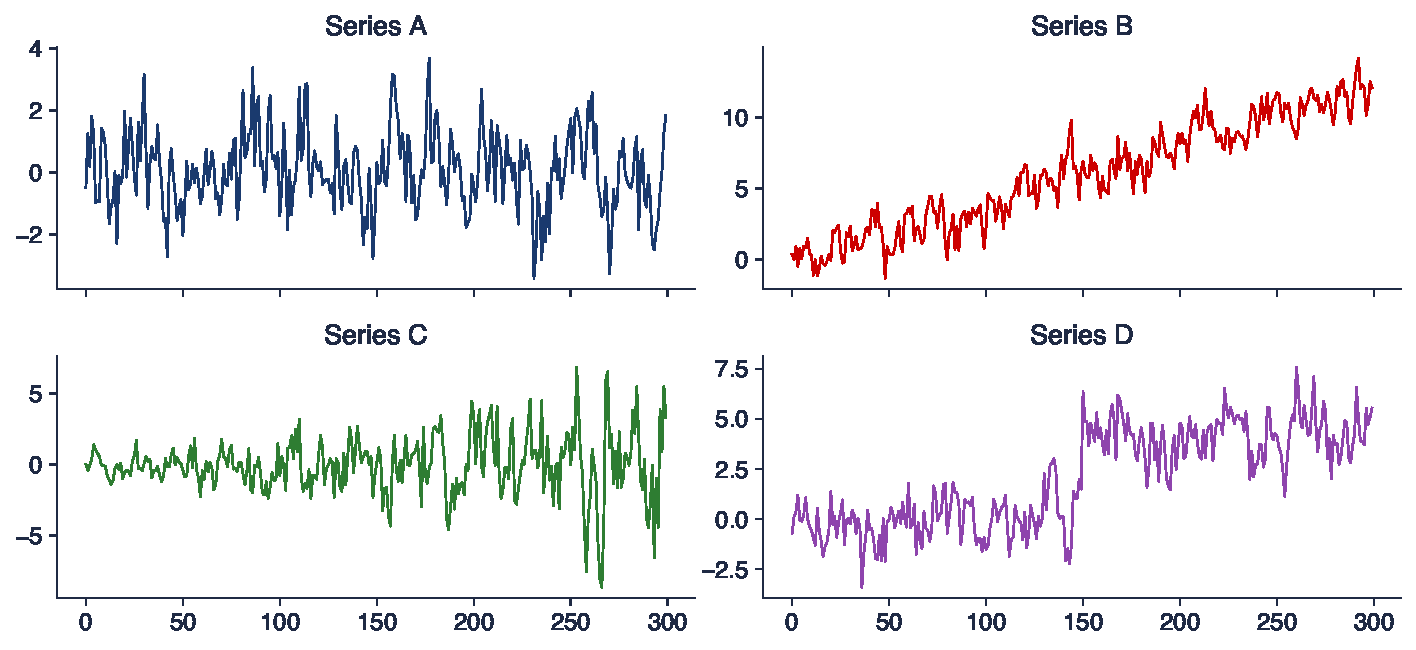
\includegraphics[width=0.97\textwidth,height=0.64\textheight,keepaspectratio]{tsa_ch1_nonstationary.pdf}
\end{center}
\vspace{-0.25cm}
\begin{itemize}
    \item Four simulated series, 300 observations each; the same AR(1) noise with $\phi = 0.5$ underlies all of them
    \item Which of the conditions (ii) and (iii) of weak stationarity fails for each series?
\end{itemize}
\quantlet{TSA\_ch1\_processes}{\qlurl{TSA_ch1_processes}}
\end{frame}

\begin{frame}{Answer: only series A is stationary}
\itemsize{\small}
\begin{itemize}
    \item \textbf{A}: stationary AR(1): constant mean and variance, the ACF depends only on the lag
    \item \textbf{B}: deterministic trend, $\mu_t = 0.04\,t$: condition (ii) fails
    \begin{itemize}
        \item a \textbf{trend-stationary} series: stationary around a line, after subtracting the trend
    \end{itemize}
    \item \textbf{C}: the standard deviation grows 7.5 times along the sample: condition (iii) fails at $h = 0$
    \item \textbf{D}: a level shift of $+4$ at $t = 150$: condition (ii) fails
    \begin{itemize}
        \item a structural break; in real data: a change of regime or of policy (the Nile, Section 8)
    \end{itemize}
    \item In practice, a plot of the series is the first check; formal tests come in \tsachlink{https://danpele.github.io/Time-Series-Analysis/EN/Courses/chapter3_unit_roots_arima_models.pdf}{Chapter 3}
\end{itemize}
\end{frame}

\begin{frame}{Recap: Stationarity}
\itemsize{\small}
\begin{itemize}
    \item Strict: all joint distributions are shift-invariant; weak: constant mean, $\gamma$ depends only on the lag
    \item Strict + finite variance $\Rightarrow$ weak; for Gaussian processes they coincide
    \item MA(1) is always stationary; AR(1) is stationary for $|\phi| < 1$, with $\rho(h) = \phi^{|h|}$
    \item Trends, changing variance and breaks violate stationarity
\end{itemize}
\end{frame}


%=============================================================================
\section{White noise and the random walk}
%=============================================================================

\begin{frame}{White noise}
\itemsize{\small}
\begin{itemize}
    \item \textbf{Definition}: $\{\varepsilon_t\}$ is \textbf{white noise}, $\varepsilon_t \sim \mathrm{WN}(0, \sigma^2)$, if
    \begin{itemize}
        \item $E[\varepsilon_t] = 0$, $\mathrm{Var}(\varepsilon_t) = \sigma^2$ and $\mathrm{Cov}(\varepsilon_t, \varepsilon_s) = 0$ for $t \ne s$
        \item so $\rho(0) = 1$ and $\rho(h) = 0$ for every $h \ne 0$
    \end{itemize}
    \item Three versions, from weakest to strongest
    \begin{itemize}
        \item \textbf{weak} white noise: only uncorrelated; non-linear dependence is allowed (for example, in the squares)
        \item \textbf{i.i.d.} (strong) white noise: independent and identically distributed
        \item \textbf{Gaussian} white noise: i.i.d. $N(0, \sigma^2)$; for jointly Normal variables, uncorrelated means independent
    \end{itemize}
    \item White noise is the building block of every model in this course: ARMA, ARIMA, GARCH, VAR
\end{itemize}
\end{frame}

\begin{frame}{Three kinds of white noise}
\itemsize{\footnotesize}
\begin{center}
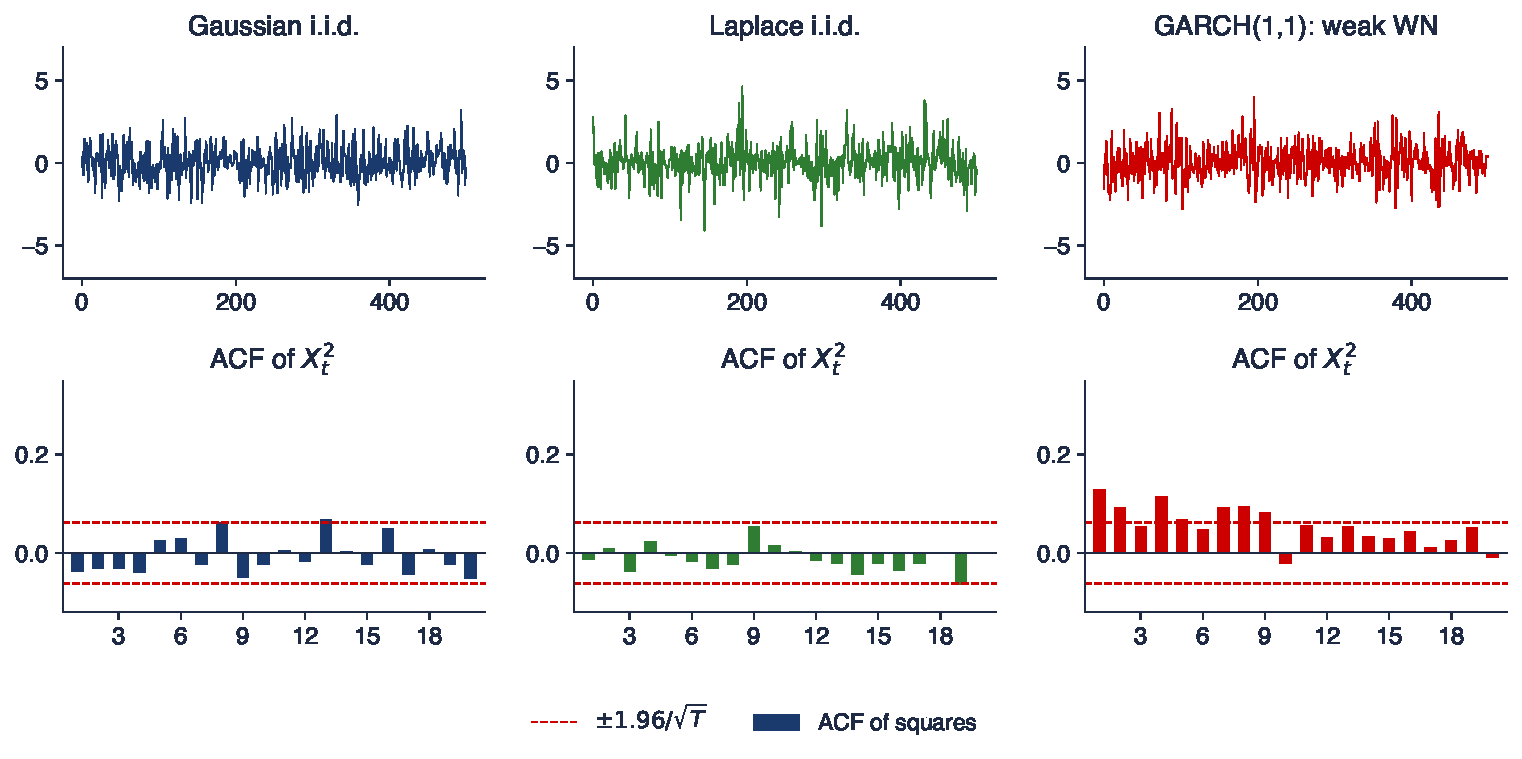
\includegraphics[width=0.97\textwidth,height=0.64\textheight,keepaspectratio]{tsa_ch1_white_noise.pdf}
\end{center}
\vspace{-0.25cm}
\begin{itemize}
    \item Top: 500 of 1000 simulated values, variance 1 in all three; bottom: the ACF of the squares $X_t^2$
    \item GARCH(1,1) (\tsachlink{https://danpele.github.io/Time-Series-Analysis/EN/Courses/chapter5_conditional_volatility_garch.pdf}{Chapter 5}): $\sigma_t^2 = 0.05 + 0.10\,\varepsilon_{t-1}^2 + 0.85\,\sigma_{t-1}^2$, $\varepsilon_t = \sigma_t z_t$; $\sigma_t^2$: the variance of day $t$ given the past; $z_t$: i.i.d. $N(0, 1)$
\end{itemize}
\quantlet{TSA\_ch1\_processes}{\qlurl{TSA_ch1_processes}}
\end{frame}

\begin{frame}{Interpreting the three white noises}
\itemsize{\small}
\begin{itemize}
    \item All three are white noise by construction; Ljung--Box $Q^*(10)$ (Section 6) on $X_t$: p = 0.278 (Gaussian), 0.986 (Laplace), 0.049 (GARCH)
    \begin{itemize}
        \item the GARCH series is close to rejection although it is uncorrelated: with changing variance the usual test rejects too often
    \end{itemize}
    \item Laplace: heavier tails (kurtosis 5.2 against 3.0), but still i.i.d.: the squares are uncorrelated (p = 0.680)
    \begin{itemize}
        \item heavy tails alone do not create dependence
    \end{itemize}
    \item GARCH: the squares are strongly correlated, $Q^*(10) = 73.2$, p $<$\,0.001
    \begin{itemize}
        \item a weak white noise: unpredictable sign and level, predictable size (volatility clustering)
        \item daily returns behave like this (BET, Section 5)
    \end{itemize}
\end{itemize}
\end{frame}

\begin{frame}{The random walk}
\itemsize{\small}
\begin{itemize}
    \item \textbf{Definition}: $X_t = X_{t-1} + \varepsilon_t$, $t \ge 1$, $X_0 = 0$, $\varepsilon_t \sim \mathrm{WN}(0, \sigma^2)$; by substitution, $X_t = \sum_{i=1}^{t}\varepsilon_i$
    \begin{itemize}
        \item every shock stays in the level forever: $\partial X_{t+h}/\partial\varepsilon_t = 1$ for all $h \ge 0$
    \end{itemize}
    \item Moments (uncorrelated shocks are enough)
    \begin{itemize}
        \item $E[X_t] = 0$; $\mathrm{Var}(X_t) = \sum_{i=1}^{t}\mathrm{Var}(\varepsilon_i) = t\sigma^2$
        \item for $t \le s$: $\mathrm{Cov}(X_t, X_s) = \mathrm{Cov}\big(\sum_{i \le t}\varepsilon_i, \sum_{j \le s}\varepsilon_j\big) = t\sigma^2$
        \item $\rho(t, s) = t/\sqrt{ts} = \sqrt{t/s}$
    \end{itemize}
    \item \textbf{Not stationary}: the variance grows with $t$, and the correlation depends on $t$, not only on $s - t$
    \begin{itemize}
        \item example: $\rho(X_{100}, X_{110}) = \sqrt{100/110} = 0.953$, but $\rho(X_{10}, X_{20}) = \sqrt{0.5} = 0.707$
    \end{itemize}
\end{itemize}
\end{frame}

\begin{frame}{Random walks and their variance}
\itemsize{\footnotesize}
\begin{center}
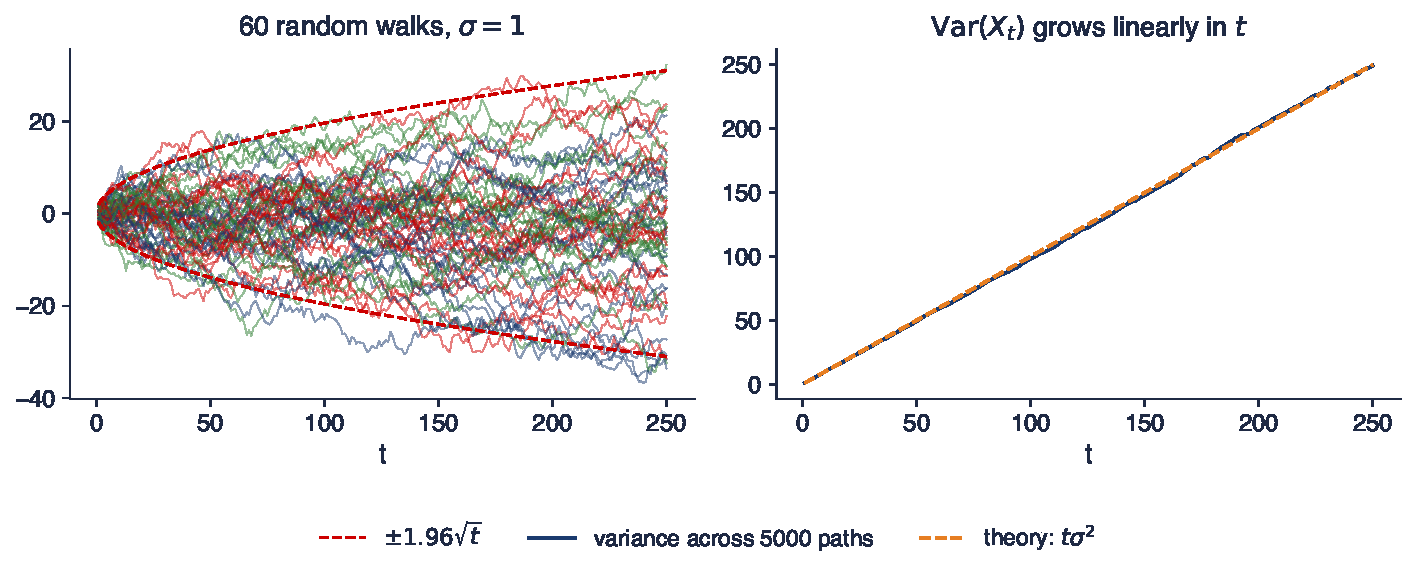
\includegraphics[width=0.97\textwidth,height=0.62\textheight,keepaspectratio]{tsa_ch1_random_walk.pdf}
\end{center}
\vspace{-0.25cm}
\begin{itemize}
    \item Left: 60 paths with $\sigma = 1$ and the band $\pm 1.96\sqrt{t}$; right: the variance of $X_t$ across 5000 paths and the line $t\sigma^2$
    \item At $t = 250$: simulated variance 249.1 (theory: 250); share of paths outside the band: 5.0\%
\end{itemize}
\quantlet{TSA\_ch1\_processes}{\qlurl{TSA_ch1_processes}}
\end{frame}

\begin{frame}{Interpreting the random walks}
\itemsize{\small}
\begin{itemize}
    \item The spread grows like $\sqrt{t}$: uncertainty about the level accumulates
    \begin{itemize}
        \item a forecast of the level 100 days ahead has variance $100\sigma^2$
    \end{itemize}
    \item Paths look like they have trends and cycles, although nothing but chance drives them
    \begin{itemize}
        \item the same lesson as \refSlutzky: sums of random shocks can look like economic cycles
    \end{itemize}
    \item Simulated $\rho(X_{100}, X_{110}) = 0.953$ against 0.953 in theory
    \begin{itemize}
        \item levels far apart in time are still highly correlated: very slow ACF decay
    \end{itemize}
\end{itemize}
\end{frame}

\begin{frame}{The random walk with drift}
\itemsize{\small}
\begin{itemize}
    \item $X_t = c + X_{t-1} + \varepsilon_t$, $X_0 = 0$: $X_t = ct + \sum_{i=1}^{t}\varepsilon_i$; $c$ is the \textbf{drift}
    \begin{itemize}
        \item $E[X_t] = ct$: a linear trend in the mean; $\mathrm{Var}(X_t) = t\sigma^2$ as before
    \end{itemize}
    \item The first difference is stationary: $\Delta X_t = X_t - X_{t-1} = c + \varepsilon_t$
    \begin{itemize}
        \item a \textbf{difference-stationary} series, with a \textbf{stochastic trend}
    \end{itemize}
    \item Compare with the trend-stationary $Y_t = a + bt + u_t$, $u_t$ stationary; $a$: intercept, $b$: slope of the trend
    \begin{itemize}
        \item both have a linear mean; in $Y_t$ shocks fade, in $X_t$ they last forever
        \item telling the two apart is the unit-root problem of \tsachlink{https://danpele.github.io/Time-Series-Analysis/EN/Courses/chapter3_unit_roots_arima_models.pdf}{Chapter 3}
    \end{itemize}
    \item Log prices of stocks and indices are often close to a random walk with a small positive drift
\end{itemize}
\end{frame}

\begin{frame}{The Bucharest Stock Exchange}
\itemsize{\small}
\begin{columns}[T]
\begin{column}{0.50\textwidth}
\centering

\includegraphics[height=0.50\textheight]{ch1_bvb_2024.jpg}\\[1mm]
\imgcap{The Bucharest Stock Exchange (BVB), 2024}
\imgcredit{https://commons.wikimedia.org/wiki/File:Bursa_de_Valori_București.jpg}{Photo: Corina Chitu (2024); CC BY-SA 4.0; Wikimedia Commons}
\end{column}
\begin{column}{0.46\textwidth}
\begin{itemize}
    \item The BET index: the reference index of the BVB (Bucharest Stock Exchange), computed since 19 September 1997
    \item Daily closes since 2000: 6\,670 log returns $r_t = 100\,\Delta\ln P_t$ ($P_t$: the closing level on day $t$); standard deviation 1.40\% per day
    \item Is the BET log price a random walk? A first, visual test on the next slide
\end{itemize}
\end{column}
\end{columns}
\end{frame}

\begin{frame}{Question for the room: which one is real?}
\itemsize{\footnotesize}
\begin{center}
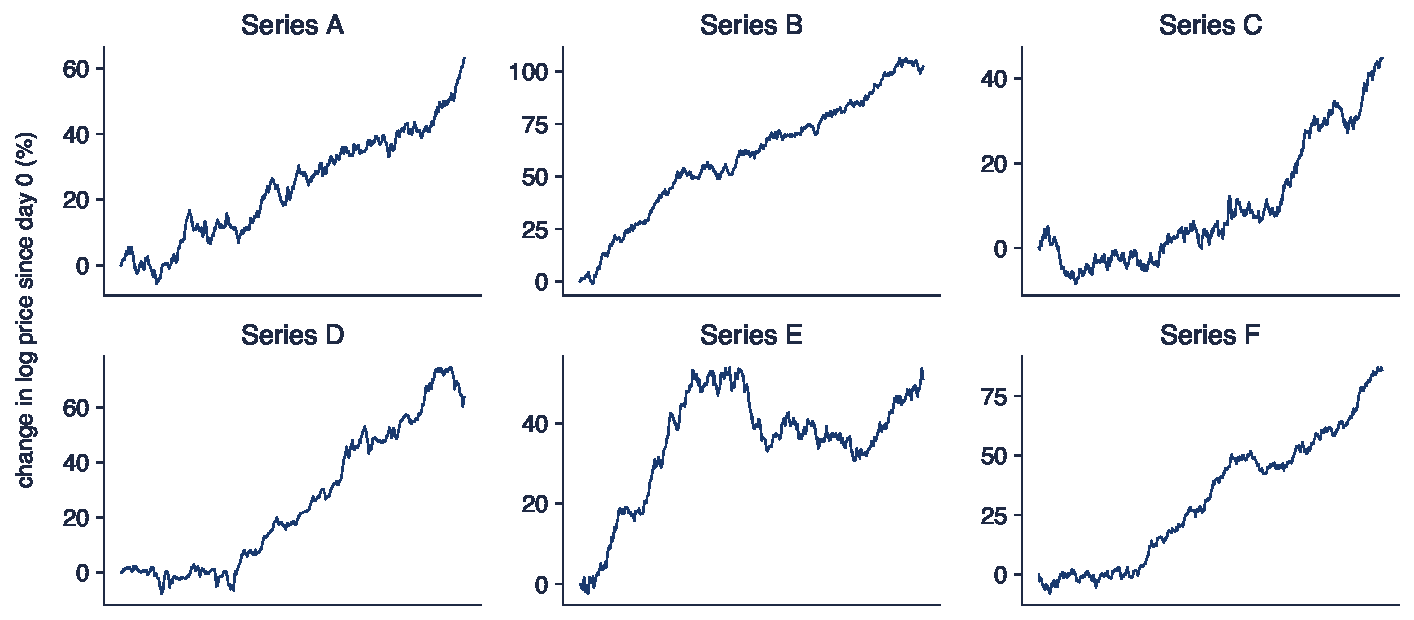
\includegraphics[width=0.97\textwidth,height=0.64\textheight,keepaspectratio]{tsa_ch1_spot_real.pdf}
\end{center}
\vspace{-0.25cm}
\begin{itemize}
    \item One panel: the BET log price over its last 500 trading days; five panels: random walks with the same drift and the same daily standard deviation
    \item Which panel is the BET?
\end{itemize}
\quantlet{TSA\_ch1\_processes}{\qlurl{TSA_ch1_processes}}
\end{frame}

\begin{frame}{Answer: series D}
\itemsize{\small}
\begin{itemize}
    \item Series D is the BET, 11 September 2024 to 18 September 2026: mean daily change 0.13\%, standard deviation 0.99\%
    \begin{itemize}
        \item by eye, it cannot be told apart from the random walks
    \end{itemize}
    \item The data are not exactly a random walk: the first-order autocorrelation of the daily changes is 0.12; Ljung--Box $Q^*(10)$ p-value 0.018
    \begin{itemize}
        \item small departures, invisible in the level, show up in the ACF of the differences
    \end{itemize}
    \item Lesson: study the changes, not the level; the tools are the ACF and the portmanteau tests (Sections 5--6)
\end{itemize}
\end{frame}

\begin{frame}{Recap: White noise and the random walk}
\itemsize{\small}
\begin{itemize}
    \item White noise: mean 0, constant variance, no autocorrelation; weak, i.i.d. or Gaussian
    \item Uncorrelated is not independent: the squares of a weak white noise can be correlated
    \item Random walk: $\mathrm{Var}(X_t) = t\sigma^2$, $\rho(t, s) = \sqrt{t/s}$: not stationary; its difference is white noise
    \item Trend-stationary and difference-stationary series look alike but react differently to shocks
\end{itemize}
\end{frame}


%=============================================================================
\section{The lag operator, differencing and the Wold decomposition}
%=============================================================================

\begin{frame}{The lag operator}
\itemsize{\small}
\begin{itemize}
    \item \textbf{Definition}: $LX_t = X_{t-1}$; powers: $L^kX_t = X_{t-k}$, $L^0 = 1$ (also written $B$, the backshift operator)
    \begin{itemize}
        \item a constant is unchanged: $Lc = c$
    \end{itemize}
    \item \textbf{Lag polynomials}: $\phi(L) = 1 - \phi_1L - \dots - \phi_pL^p$
    \begin{itemize}
        \item $p$: the degree (the largest lag); $\phi_1, \dots, \phi_p$: real coefficients; $\phi(L)X_t = X_t - \phi_1X_{t-1} - \dots - \phi_pX_{t-p}$
        \item AR(1): $(1 - \phi L)X_t = \varepsilon_t$; MA(1): $X_t = (1 + \theta L)\varepsilon_t$
        \item they multiply like ordinary polynomials: $(1 - L)(1 + L) = 1 - L^2$
    \end{itemize}
    \item \textbf{Inversion}: for $|\phi| < 1$, $(1 - \phi L)^{-1} = 1 + \phi L + \phi^2L^2 + \dots$ (a geometric series)
    \begin{itemize}
        \item so the AR(1) is $X_t = \sum_{j \ge 0}\phi^j\varepsilon_{t-j}$: an infinite moving average
    \end{itemize}
    \item The language of \tsachlink{https://danpele.github.io/Time-Series-Analysis/EN/Courses/chapter2_arma_models.pdf}{Chapters 2}--\tsachlink{https://danpele.github.io/Time-Series-Analysis/EN/Courses/chapter4_seasonality_forecasting.pdf}{4}: ARMA, ARIMA and SARIMA models are written with lag polynomials
\end{itemize}
\end{frame}

\begin{frame}{Differencing}
\itemsize{\small}
\begin{itemize}
    \item \textbf{First difference}: $\Delta X_t = (1 - L)X_t = X_t - X_{t-1}$; \textbf{second}: $\Delta^2X_t = (1 - L)^2X_t = X_t - 2X_{t-1} + X_{t-2}$
    \begin{itemize}
        \item \textbf{seasonal difference} with period $s$: $\Delta_sX_t = (1 - L^s)X_t = X_t - X_{t-s}$ ($s = 4$ for quarters, $s = 12$ for months)
    \end{itemize}
    \item \textbf{Worked example}: $x = (10, 12, 15, 14, 18)$
    \begin{itemize}
        \item $\Delta x = (2, 3, -1, 4)$; $\Delta^2x = (1, -4, 5)$; each difference loses one observation
    \end{itemize}
    \item What differencing removes
    \begin{itemize}
        \item a linear trend: $\Delta(a + bt) = b$; a quadratic trend needs $\Delta^2$
        \item a random walk: $\Delta X_t = \varepsilon_t$; a seasonal pattern that repeats exactly: $\Delta_s$
    \end{itemize}
    \item \textbf{Integrated process}: $X_t \sim I(d)$ if $\Delta^dX_t$ is stationary and $\Delta^{d-1}X_t$ is not
    \begin{itemize}
        \item white noise is $I(0)$, the random walk is $I(1)$; testing $d$: \tsachlink{https://danpele.github.io/Time-Series-Analysis/EN/Courses/chapter3_unit_roots_arima_models.pdf}{Chapter 3}
    \end{itemize}
\end{itemize}
\end{frame}

\begin{frame}{S\&P 500: the level and its difference}
\itemsize{\footnotesize}
\begin{center}
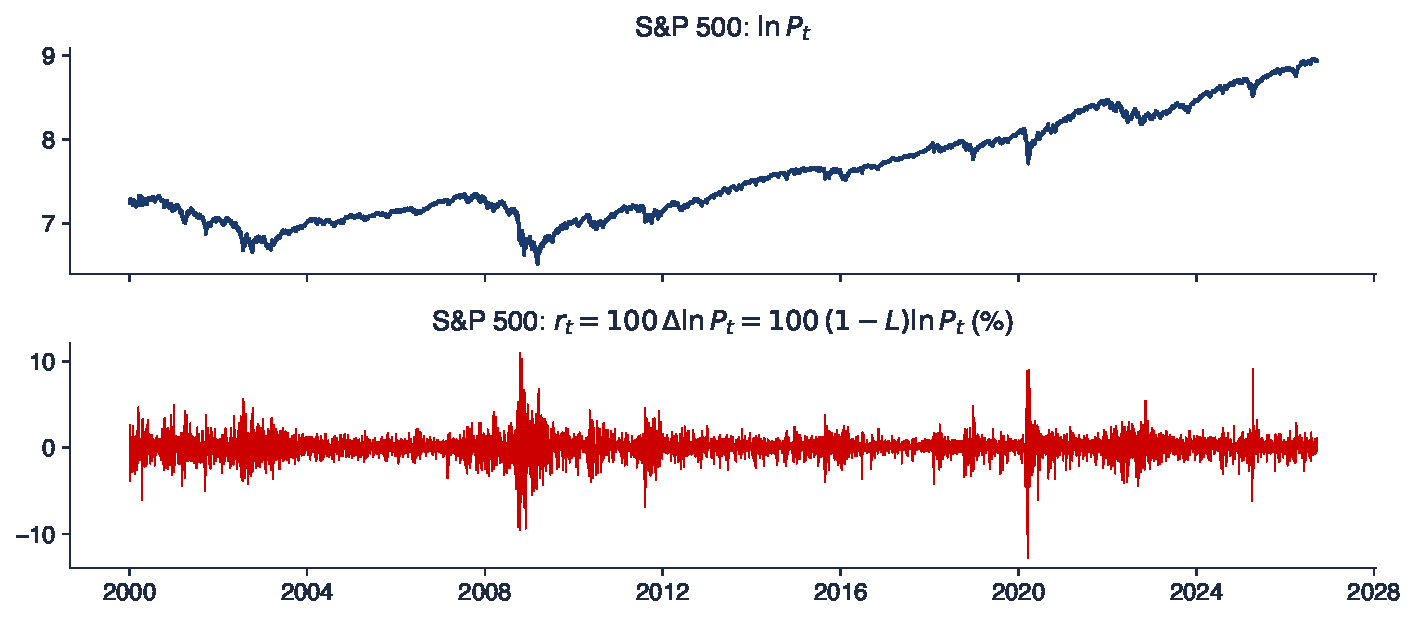
\includegraphics[width=0.97\textwidth,height=0.66\textheight,keepaspectratio]{tsa_ch1_sp500_diff.pdf}
\end{center}
\vspace{-0.25cm}
\begin{itemize}
    \item Top: the log of the S\&P 500 index since 2000; bottom: the daily log returns, 6\,714 days to 18 September 2026
\end{itemize}
\quantlet{TSA\_ch1\_transformations}{\qlurl{TSA_ch1_transformations}}
\end{frame}

\begin{frame}{Interpreting the S\&P 500 transformation}
\itemsize{\small}
\begin{itemize}
    \item Log price: sample ACF 0.999 at lag 1 and still 0.973 at lag 50
    \begin{itemize}
        \item the behaviour of a random walk: the level remembers everything
    \end{itemize}
    \item Log returns: mean 0.025\% per day, standard deviation 1.21\%; ACF at lag 1: $\ensuremath{-}0.099$
    \begin{itemize}
        \item a constant level: one difference removed the stochastic trend
    \end{itemize}
    \item Not yet white noise in the strict sense: quiet and turbulent periods alternate (2008, 2020)
    \begin{itemize}
        \item the returns are close to a weak white noise; their variance is the subject of \tsachlink{https://danpele.github.io/Time-Series-Analysis/EN/Courses/chapter5_conditional_volatility_garch.pdf}{Chapter 5}
    \end{itemize}
\end{itemize}
\end{frame}

\begin{frame}{The Wold decomposition}
\itemsize{\footnotesize}
\begin{columns}[T]
\begin{column}{0.66\textwidth}
\begin{itemize}
    \item \textbf{Theorem} \refWold: every weakly stationary process with mean 0 can be written as
    \begin{itemize}
        \item $X_t = \sum_{j=0}^{\infty}\psi_j\varepsilon_{t-j} + \eta_t$, with $\psi_0 = 1$, $\sum_j\psi_j^2 < \infty$
        \item $\varepsilon_t$: white noise, the error of the best linear forecast of $X_t$ from its past (the \textbf{innovation})
        \item $\eta_t$: a deterministic part, perfectly predictable from the distant past (for example, a fixed cycle)
    \end{itemize}
    \item Meaning
    \begin{itemize}
        \item any stationary series is a weighted sum of past shocks: MA($\infty$)
        \item the weights $\psi_j$ = the effect of a shock after $j$ periods (impulse response)
        \item ARMA models (\tsachlink{https://danpele.github.io/Time-Series-Analysis/EN/Courses/chapter2_arma_models.pdf}{Chapter 2}) approximate the infinite $\psi_j$ with few parameters
    \end{itemize}
\end{itemize}
\end{column}
\begin{column}{0.30\textwidth}
\centering
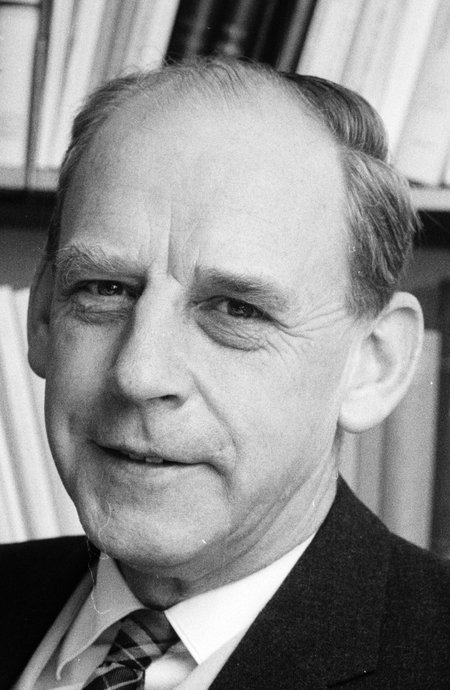
\includegraphics[height=0.48\textheight]{ch1_herman_wold_1969.jpg}\\[1mm]
\imgcap{Herman Wold, Uppsala, 1969}
\imgcredit{https://commons.wikimedia.org/wiki/File:Professor_Herman_Wold,_Uppsala,_1969_(cropped).jpg}{Photo: Uppsala-Bild (1969); CC BY 4.0; Wikimedia Commons}
\end{column}
\end{columns}
\end{frame}

\begin{frame}{Wold weights of four processes}
\itemsize{\footnotesize}
\begin{center}
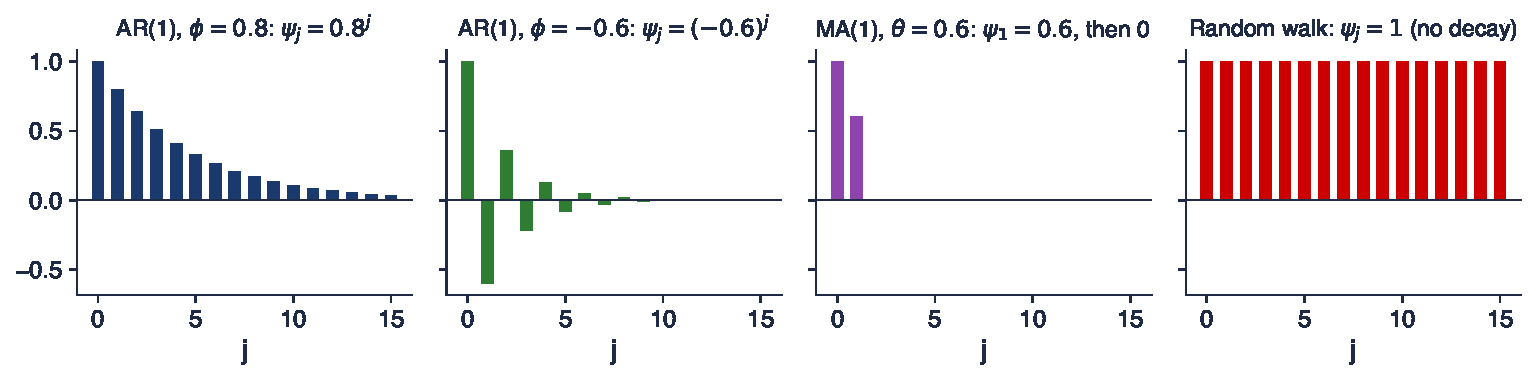
\includegraphics[width=0.97\textwidth,height=0.50\textheight,keepaspectratio]{tsa_ch1_wold.pdf}
\end{center}
\vspace{-0.25cm}
\begin{itemize}
    \item $\psi_j$, $j = 0, \dots, 15$: AR(1) with $\phi = 0.8$ and $\phi = -0.6$, MA(1) with $\theta = 0.6$, and the random walk
    \item AR(1), $\phi = 0.8$: $\psi_5 = 0.328$, $\psi_{10} = 0.107$; $\mathrm{Var}(X_t) = \sigma^2\sum_j\psi_j^2 = 2.78\,\sigma^2$
\end{itemize}
\quantlet{TSA\_ch1\_wold\_ergodicity}{\qlurl{TSA_ch1_wold_ergodicity}}
\end{frame}

\begin{frame}{Interpreting the Wold weights}
\itemsize{\small}
\begin{itemize}
    \item Stationary processes: $\psi_j \to 0$, so shocks fade and the variance $\sigma^2\sum_j\psi_j^2$ is finite
    \begin{itemize}
        \item $\phi < 0$: the effect alternates in sign; MA(1): the effect stops after one period
    \end{itemize}
    \item Random walk: $\psi_j = 1$ for all $j$, $\sum_j\psi_j^2 = \infty$: no Wold form, no stationarity
    \begin{itemize}
        \item the economic meaning: a permanent shock (a technology shock to GDP, news in a price)
    \end{itemize}
    \item The ACF is fixed by the weights: $\gamma(h) = \sigma^2\sum_j\psi_j\psi_{j+h}$
\end{itemize}
\end{frame}

\begin{frame}{Ergodicity}
\itemsize{\small}
\begin{itemize}
    \item Stationarity says the moments are constant; we still need to estimate them from \textbf{one} path
    \begin{itemize}
        \item ensemble mean: $\mu = E[X_t]$ (across paths); time mean: $\bar X_T = \frac1T\sum_{t=1}^{T}X_t$ (along one path)
    \end{itemize}
    \item \textbf{Definition}: a stationary process is \textbf{ergodic for the mean} if $\bar X_T \to \mu$ (in mean square) as $T \to \infty$
    \begin{itemize}
        \item a sufficient condition: $\gamma(h) \to 0$ as $h \to \infty$ (correlation dies out)
        \item if $\sum_h|\gamma(h)| < \infty$, then $T\,\mathrm{Var}(\bar X_T) \to \sum_{h=-\infty}^{\infty}\gamma(h)$
    \end{itemize}
    \item \textbf{Counterexample}: $X_t = Z + \varepsilon_t$, $Z \sim N(0, 1)$ drawn once, $\varepsilon_t$ white noise
    \begin{itemize}
        \item stationary, with $\gamma(h) = 1$ for every $h \ne 0$; $\bar X_T \to Z$, not $\mu = 0$
    \end{itemize}
\end{itemize}
\end{frame}

\begin{frame}{Time averages: ergodic and non-ergodic}
\itemsize{\footnotesize}
\begin{center}
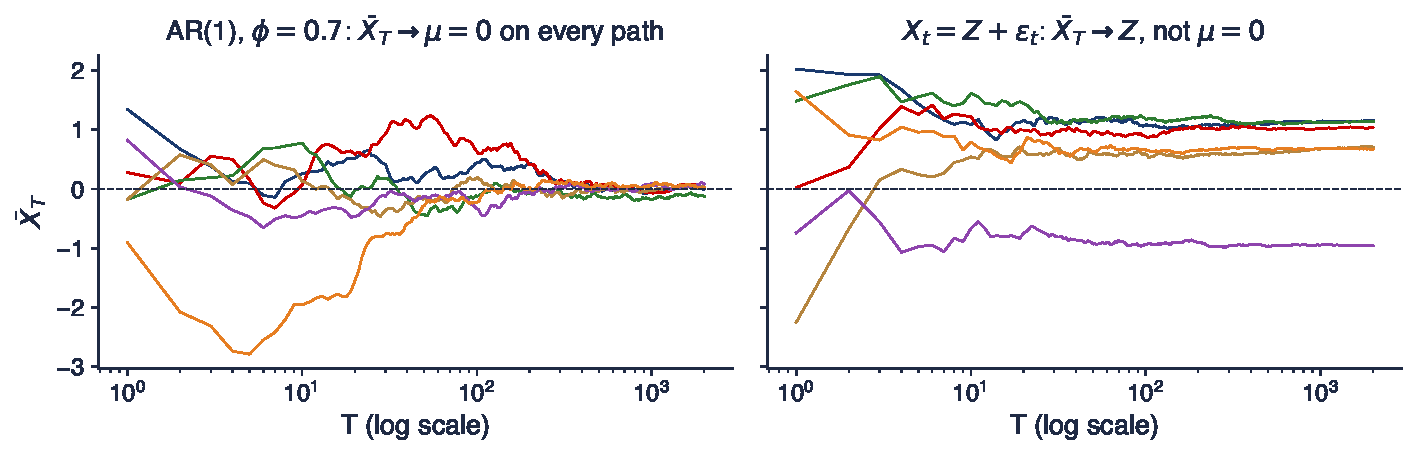
\includegraphics[width=0.97\textwidth,height=0.58\textheight,keepaspectratio]{tsa_ch1_ergodicity.pdf}
\end{center}
\vspace{-0.25cm}
\begin{itemize}
    \item Running mean $\bar X_T$ along 6 paths, $T$ up to 2\,000: AR(1) with $\phi = 0.7$ (left) and $X_t = Z + \varepsilon_t$ (right)
    \item Final values: between $\ensuremath{-}0.13$ and $0.09$ on the left; between $\ensuremath{-}0.95$ and $1.16$ on the right, close to the drawn $Z$
\end{itemize}
\quantlet{TSA\_ch1\_wold\_ergodicity}{\qlurl{TSA_ch1_wold_ergodicity}}
\end{frame}

\begin{frame}{Interpreting ergodicity}
\itemsize{\small}
\begin{itemize}
    \item Left: every path ``learns'' the true mean 0; one long history is as good as many histories
    \begin{itemize}
        \item convergence is slow when the correlation is strong: $\mathrm{Var}(\bar X_T) \approx \gamma(0)(1 + \phi)/((1 - \phi)T)$
    \end{itemize}
    \item Right: each path converges to its own $Z$; no amount of data from one path reveals $\mu = 0$
    \begin{itemize}
        \item an economy with a permanent, unobserved ``type'' behaves like this
    \end{itemize}
    \item Ergodicity cannot be tested from one path; it is assumed whenever we estimate moments from a single series
\end{itemize}
\end{frame}

\begin{frame}{Recap: The lag operator, differencing and Wold}
\itemsize{\small}
\begin{itemize}
    \item $L^kX_t = X_{t-k}$; $\Delta = 1 - L$; $\Delta_s = 1 - L^s$; $I(d)$: stationary after $d$ differences
    \item Wold: a stationary process is an MA($\infty$) of its innovations, with $\sum\psi_j^2 < \infty$
    \item Ergodicity lets time averages estimate ensemble moments; it needs correlations that die out
\end{itemize}
\end{frame}


%=============================================================================
\section{Sample ACF and PACF}
%=============================================================================

\begin{frame}{Sample autocovariance and autocorrelation}
\itemsize{\small}
\begin{itemize}
    \item From $x_1, \dots, x_T$, with the sample mean $\bar x = \frac1T\sum_t x_t$:
    \begin{itemize}
        \item $\hat\gamma(h) = \frac1T\sum_{t=1}^{T-h}(x_t - \bar x)(x_{t+h} - \bar x)$, $0 \le h < T$
        \item $\hat\rho(h) = \hat\gamma(h)/\hat\gamma(0)$: the \textbf{sample ACF}; the plot of $\hat\rho(h)$ against $h$ is the \textbf{correlogram}
    \end{itemize}
    \item Why divide by $T$ and not by $T - h$?
    \begin{itemize}
        \item the sequence $\hat\gamma(h)$ is then non-negative definite, like a true autocovariance \refBD
        \item the price: a small bias towards 0 at large lags; use $h \le T/4$
    \end{itemize}
    \item \textbf{Worked example}: $x = (3, 5, 4, 6, 7)$, $\bar x = 5$, deviations $(-2, 0, -1, 1, 2)$
    \begin{itemize}
        \item $\hat\gamma(0) = 10/5 = 2.0$; $\hat\gamma(1) = (0 + 0 - 1 + 2)/5 = 0.2$; $\hat\gamma(2) = (2 + 0 - 2)/5 = 0.0$
        \item $\hat\rho(1) = 0.10$, $\hat\rho(2) = 0.00$; with $T = 5$ the band is $\pm 0.88$: far too few data
    \end{itemize}
\end{itemize}
\end{frame}

\begin{frame}{Confidence bands for the sample ACF}
\itemsize{\small}
\begin{itemize}
    \item \textbf{Large-sample result} of \refBartlett: if $X_t$ is i.i.d. with finite variance, for large $T$
    \begin{itemize}
        \item $\hat\rho(1), \dots, \hat\rho(m)$ are approximately independent $N(0, 1/T)$
        \item 95\% band: $\pm 1.96/\sqrt{T}$; a bar outside it rejects $\rho(h) = 0$ at 5\%, \textbf{for that lag alone}
    \end{itemize}
    \item For an MA($q$), at lags $h > q$: $\mathrm{Var}(\hat\rho(h)) \approx \frac1T\big(1 + 2\sum_{k=1}^{q}\rho(k)^2\big)$
    \begin{itemize}
        \item the wider bands of \texttt{statsmodels} \texttt{plot\_acf} (\tsachlink{https://danpele.github.io/Time-Series-Analysis/EN/Courses/chapter2_arma_models.pdf}{Chapter 2})
    \end{itemize}
    \item Two traps
    \begin{itemize}
        \item with 20 lags and no correlation, about one bar is expected outside the band by chance
        \item the band assumes i.i.d. data; for a weak white noise (GARCH returns) the true band is wider
    \end{itemize}
\end{itemize}
\end{frame}

\begin{frame}{Sampling distribution of the sample ACF}
\itemsize{\footnotesize}
\begin{center}
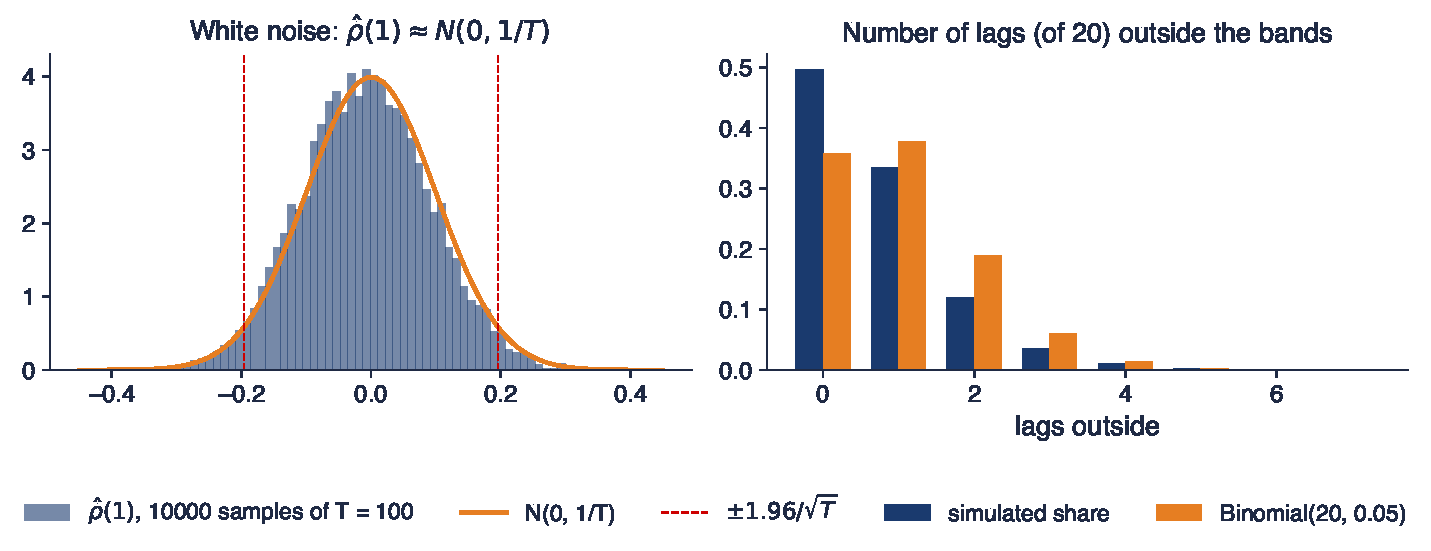
\includegraphics[width=0.97\textwidth,height=0.60\textheight,keepaspectratio]{tsa_ch1_bartlett.pdf}
\end{center}
\vspace{-0.25cm}
\begin{itemize}
    \item 10000 samples of Gaussian white noise with $T = 100$: $\hat\rho(1)$ (left) and the number of lags, out of 20, outside $\pm 0.196$ (right)
\end{itemize}
\quantlet{TSA\_ch1\_acf\_pacf}{\qlurl{TSA_ch1_acf_pacf}}
\end{frame}

\begin{frame}{Interpreting the simulation}
\itemsize{\small}
\begin{itemize}
    \item $\hat\rho(1)$: mean $\ensuremath{-}0.008$ (theory $-1/T = -0.01$), standard deviation 0.098 (theory $1/\sqrt{T} = 0.1$)
    \begin{itemize}
        \item Bartlett's approximation is already good at $T = 100$
    \end{itemize}
    \item At least one of 20 bars outside the band in 50\% of the samples, although there is no correlation at all
    \begin{itemize}
        \item independent tests would give $1 - 0.95^{20} = 64\%$; at distant lags $\mathrm{Var}(\hat\rho(h)) < 1/T$, so slightly fewer bars cross
    \end{itemize}
    \item Do not over-read single bars: judge the pattern, or use a joint test (Section 6)
\end{itemize}
\end{frame}

\begin{frame}{Theoretical and sample ACF of four processes}
\itemsize{\footnotesize}
\begin{center}
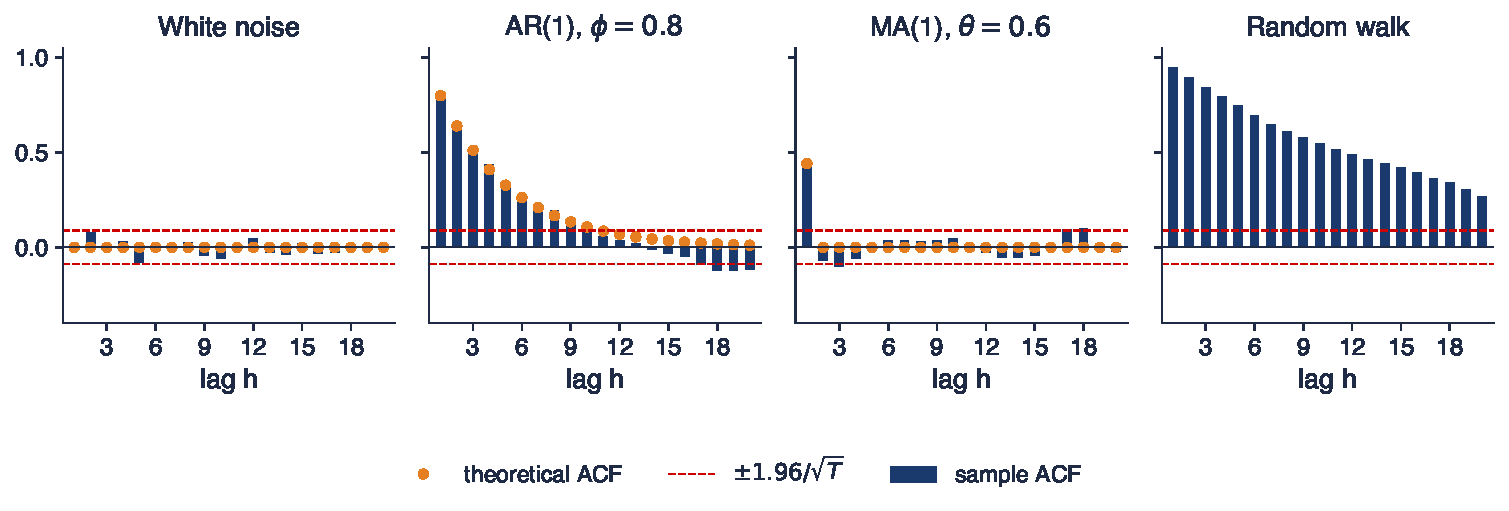
\includegraphics[width=0.97\textwidth,height=0.56\textheight,keepaspectratio]{tsa_ch1_acf_models.pdf}
\end{center}
\vspace{-0.25cm}
\begin{itemize}
    \item $T = 500$ simulated values; bars: sample ACF; dots: theoretical ACF; band $\pm 0.088$
\end{itemize}
\quantlet{TSA\_ch1\_acf\_pacf}{\qlurl{TSA_ch1_acf_pacf}}
\end{frame}

\begin{frame}{Interpreting the four correlograms}
\itemsize{\small}
\begin{itemize}
    \item White noise: all bars small; the largest, $\hat\rho(2) = 0.08$, is noise
    \item AR(1), $\phi = 0.8$: geometric decay, $\hat\rho(1) = 0.81$, $\hat\rho(2) = 0.65$ (theory 0.80 and 0.64)
    \item MA(1), $\theta = 0.6$: one spike, $\hat\rho(1) = 0.44$ (theory 0.44), then nothing: the ACF \textbf{cuts off} after lag 1
    \item Random walk: $\hat\rho(1) = 0.95$, still 0.55 at lag 10: the slow, almost linear decay of a non-stationary series
    \begin{itemize}
        \item the sample ACF of a random walk has no theoretical counterpart: $\rho(h)$ is not defined
    \end{itemize}
\end{itemize}
\end{frame}

\begin{frame}{Partial autocorrelation}
\itemsize{\small}
\begin{itemize}
    \item \textbf{Definition}: the \textbf{PACF} at lag $h$, $\phi_{hh}$, is the last coefficient of the best linear predictor of $X_t$ from $X_{t-1}, \dots, X_{t-h}$:
    \begin{itemize}
        \item $X_t = \phi_{h1}X_{t-1} + \dots + \phi_{hh}X_{t-h} + e_t$; $\phi_{h1}, \dots, \phi_{hh}$: the coefficients of the regression on $h$ lags; $e_t$: the prediction error
        \item the correlation of $X_t$ and $X_{t-h}$ after removing the linear effect of the lags in between
    \end{itemize}
    \item First two values
    \begin{itemize}
        \item $\phi_{11} = \rho(1)$; $\phi_{22} = \dfrac{\rho(2) - \rho(1)^2}{1 - \rho(1)^2}$
        \item the general case: the Durbin--Levinson recursion; the sample PACF uses $\hat\rho(h)$ in place of $\rho(h)$
    \end{itemize}
    \item \textbf{Worked example}
    \begin{itemize}
        \item AR(1): $\rho(2) = \rho(1)^2$, so $\phi_{22} = 0$: once $X_{t-1}$ is known, $X_{t-2}$ adds nothing
        \item AR(2) with $\phi_1 = 0.5$, $\phi_2 = 0.3$: $\rho(1) = 0.714$, $\rho(2) = 0.657$, $\phi_{22} = (0.657 - 0.510)/(1 - 0.510) = 0.300 = \phi_2$
    \end{itemize}
    \item Same band as the ACF under white noise: $\pm 1.96/\sqrt{T}$
\end{itemize}
\end{frame}

\begin{frame}{ACF and PACF of three processes}
\itemsize{\footnotesize}
\begin{center}
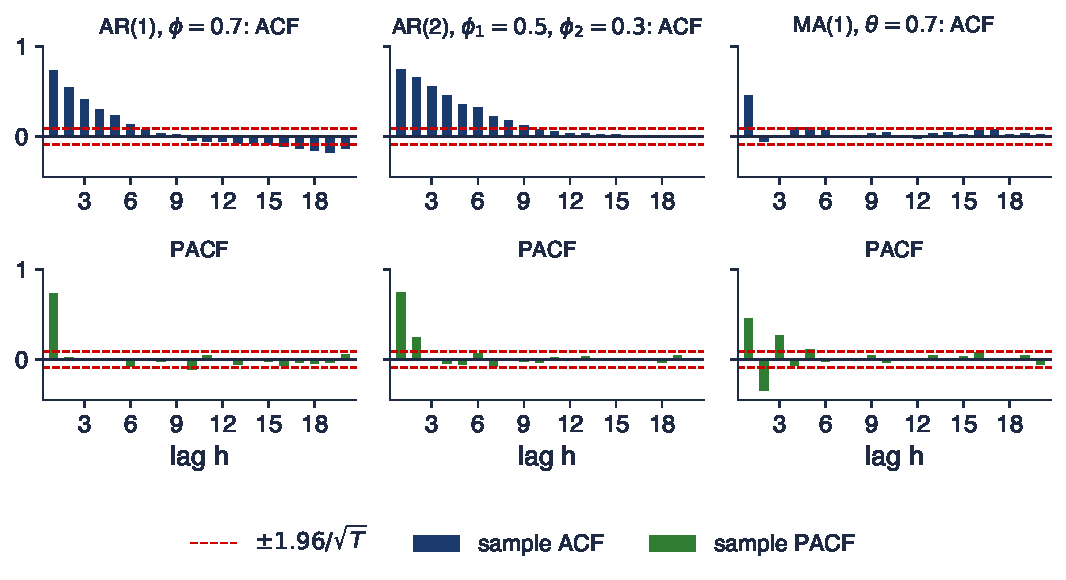
\includegraphics[width=0.97\textwidth,height=0.64\textheight,keepaspectratio]{tsa_ch1_acf_pacf.pdf}
\end{center}
\vspace{-0.25cm}
\begin{itemize}
    \item $T = 500$ simulated values of AR(1), AR(2) and MA(1); top: sample ACF; bottom: sample PACF
\end{itemize}
\quantlet{TSA\_ch1\_acf\_pacf}{\qlurl{TSA_ch1_acf_pacf}}
\end{frame}

\begin{frame}{Interpreting the ACF and PACF}
\itemsize{\small}
\begin{itemize}
    \item AR(1): the ACF decays; the PACF has one spike, $\hat\phi_{11} = 0.73$, then $\hat\phi_{22} = 0.03$
    \begin{itemize}
        \item AR(2): two PACF spikes, $\hat\phi_{22} = 0.24$ (theory 0.3), then $\hat\phi_{33} = 0.01$
    \end{itemize}
    \item MA(1): the mirror image; one ACF spike ($\hat\rho(1) = 0.46$), a PACF that alternates and decays ($\ensuremath{-}0.34$, $0.26$, ...)
    \item The identification rule of \tsachlink{https://danpele.github.io/Time-Series-Analysis/EN/Courses/chapter2_arma_models.pdf}{Chapter 2} \refHP:
    \begin{itemize}
        \item PACF cuts off after $p$: AR($p$); ACF cuts off after $q$: MA($q$); both decay: ARMA
    \end{itemize}
\end{itemize}
\end{frame}

\begin{frame}{Real data: three markets}
\itemsize{\small}
\begin{columns}[T]
\begin{column}{0.40\textwidth}
\centering
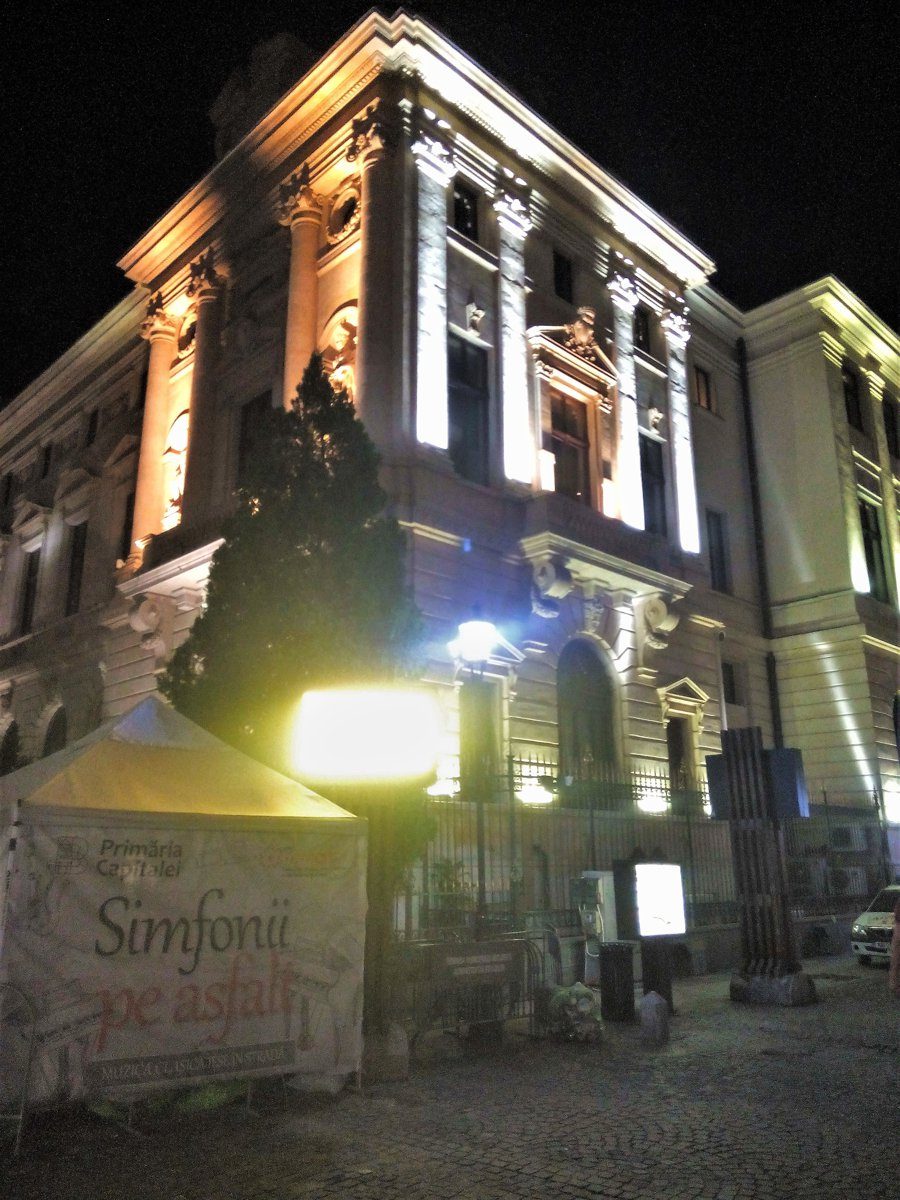
\includegraphics[height=0.48\textheight]{ch1_bnr_2018.jpg}\\[1mm]
\imgcap{The National Bank of Romania (BNR), publisher of the EUR/RON reference rate}
\imgcredit{https://commons.wikimedia.org/wiki/File:National_Bank_of_Romania_(old_building),_Bucharest_by_nickispeaki_01.jpg}{Photo: Nickispeaki (2018); CC BY-SA 4.0; Wikimedia Commons}
\end{column}
\begin{column}{0.56\textwidth}
\begin{itemize}
    \item Next: the ACF of BET daily log returns since 2000, of their absolute values and of their squares
    \item The same analysis for EUR/RON (the BNR reference rate) and the S\&P 500: Seminar 1, task B2
    \item Question: are BET returns white noise? Of which kind?
\end{itemize}
\end{column}
\end{columns}
\end{frame}

\begin{frame}{BET: ACF of returns, absolute and squared returns}
\itemsize{\footnotesize}
\begin{center}
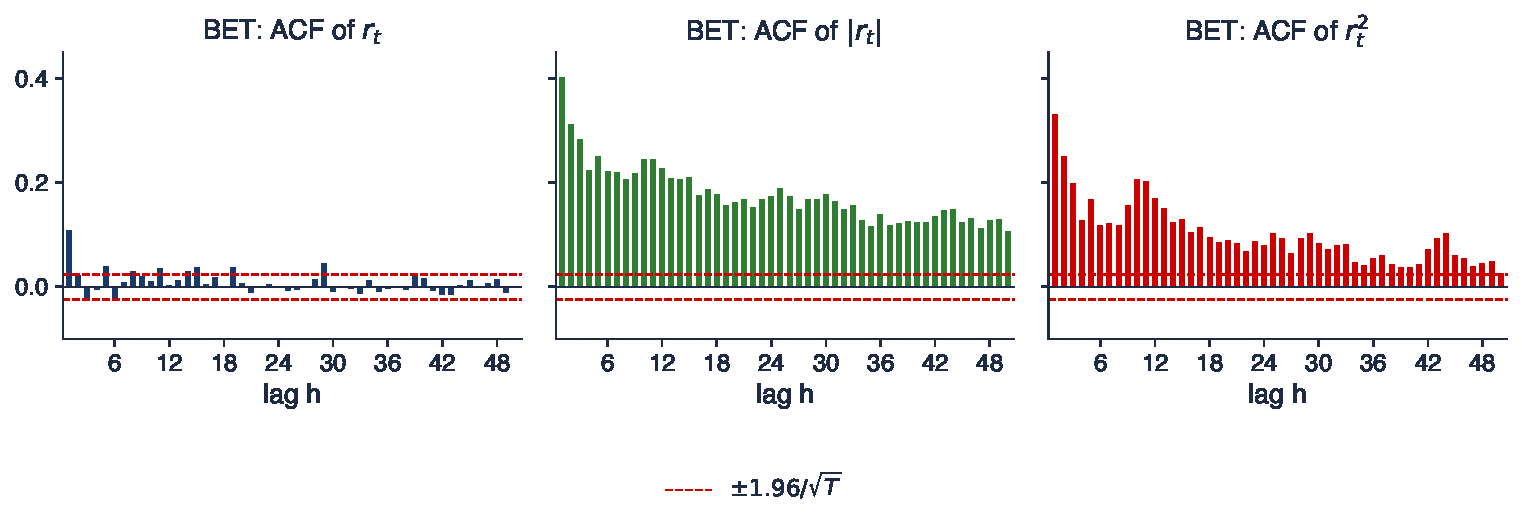
\includegraphics[width=0.97\textwidth,height=0.58\textheight,keepaspectratio]{tsa_ch1_bet_acf.pdf}
\end{center}
\vspace{-0.25cm}
\begin{itemize}
    \item Daily log returns, 6\,670 days, lags 1--50; band $\pm 0.024$
\end{itemize}
\quantlet{TSA\_ch1\_acf\_pacf}{\qlurl{TSA_ch1_acf_pacf}}
\end{frame}

\begin{frame}{Interpreting the BET correlograms}
\itemsize{\small}
\begin{itemize}
    \item Returns: $\hat\rho(1) = 0.109$, clearly outside the band; $Q^*(10) = 108$
    \begin{itemize}
        \item statistically significant but small: yesterday's return explains about $\hat\rho(1)^2 = 1.2\%$ of today's variance
        \item a typical sign of a less liquid market (non-synchronous trading)
    \end{itemize}
    \item Absolute returns: $\hat\rho(1) = 0.40$ and still 0.11 at lag 50; squares: $\hat\rho(1) = 0.33$
    \begin{itemize}
        \item large moves follow large moves: volatility clustering, a long memory in the size of returns
    \end{itemize}
    \item Conclusion: BET returns are close to a \textbf{weak} white noise; the mean is hardly predictable, the variance is (\tsachlink{https://danpele.github.io/Time-Series-Analysis/EN/Courses/chapter5_conditional_volatility_garch.pdf}{Chapter 5})
\end{itemize}
\end{frame}

\begin{frame}{Recap: Sample ACF and PACF}
\itemsize{\small}
\begin{itemize}
    \item $\hat\rho(h) = \hat\gamma(h)/\hat\gamma(0)$, with divisor $T$; use lags up to about $T/4$
    \item Under i.i.d. data: $\hat\rho(h) \approx N(0, 1/T)$, band $\pm 1.96/\sqrt{T}$; 1 bar in 20 crosses by chance
    \item PACF: direct effect of lag $h$; AR($p$) cuts off in the PACF, MA($q$) in the ACF
    \item Returns: small linear, strong non-linear dependence
\end{itemize}
\end{frame}


%=============================================================================
\section{Portmanteau tests: Box--Pierce and Ljung--Box}
%=============================================================================

\begin{frame}{Testing many autocorrelations at once}
\itemsize{\small}
\begin{itemize}
    \item $H_0$: $\rho(1) = \dots = \rho(m) = 0$ (the series is white noise up to lag $m$); $H_1$: at least one $\rho(h) \ne 0$
    \begin{itemize}
        \item a \textbf{portmanteau} test: one statistic ``carries'' $m$ autocorrelations
    \end{itemize}
    \item The \textbf{Box--Pierce statistic}, from \refBP: $Q(m) = T\sum_{h=1}^{m}\hat\rho(h)^2$
    \begin{itemize}
        \item under $H_0$, each $\sqrt{T}\hat\rho(h) \approx N(0, 1)$, independent: the sum of $m$ squares is $\approx \chi^2(m)$
    \end{itemize}
    \item The \textbf{Ljung--Box statistic}, from \refLB: $Q^*(m) = T(T + 2)\sum_{h=1}^{m}\dfrac{\hat\rho(h)^2}{T - h}$
    \begin{itemize}
        \item the weight $(T + 2)/(T - h)$ corrects the small variance of $\hat\rho(h)$ at distant lags; same $\chi^2(m)$ limit
    \end{itemize}
    \item Reject $H_0$ at 5\% if $Q^* > \chi^2_{0.95}(m)$; for example $\chi^2_{0.95}(10) = 18.31$
    \begin{itemize}
        \item $\chi^2(m)$: the chi-square distribution with $m$ degrees of freedom; $\chi^2_{0.95}(m)$: its 95\% quantile
        \item p-value: the probability under $H_0$ of a statistic at least as large as the observed one; reject if it is below 0.05
        \item on residuals of an ARMA($p, q$): $\chi^2(m - p - q)$ (\tsachlink{https://danpele.github.io/Time-Series-Analysis/EN/Courses/chapter2_arma_models.pdf}{Chapter 2})
    \end{itemize}
\end{itemize}
\end{frame}

\begin{frame}{Worked example: the Ljung--Box statistic}
\itemsize{\small}
\begin{itemize}
    \item $T = 100$; $\hat\rho(1) = 0.25$, $\hat\rho(2) = 0.12$, $\hat\rho(3) = -0.08$; band $\pm 0.196$
    \begin{itemize}
        \item only $\hat\rho(1)$ is outside the band
    \end{itemize}
    \item Box--Pierce: $Q(3) = 100\,(0.0625 + 0.0144 + 0.0064) = 8.33$
    \begin{itemize}
        \item Ljung--Box: $Q^*(3) = 100 \cdot 102\,\big(\frac{0.0625}{99} + \frac{0.0144}{98} + \frac{0.0064}{97}\big) = 8.61$
    \end{itemize}
    \item Critical value $\chi^2_{0.95}(3) = 7.81$: reject $H_0$; p-value 0.035
    \begin{itemize}
        \item the series is not white noise; the dependence is concentrated at lag 1
    \end{itemize}
    \item Choice of $m$: too small misses distant lags; too large dilutes the evidence
    \begin{itemize}
        \item common choices: $m = 10$ for non-seasonal data, $m = 2s$ for seasonal data with period $s$ \refFPP
    \end{itemize}
\end{itemize}
\end{frame}

\begin{frame}{Box--Pierce and Ljung--Box in small samples}
\itemsize{\footnotesize}
\begin{center}
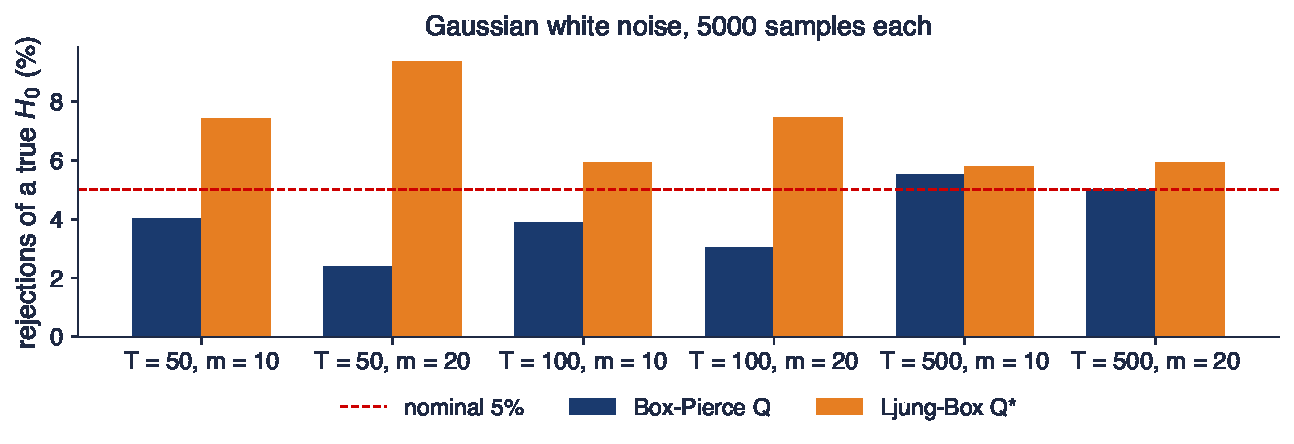
\includegraphics[width=0.97\textwidth,height=0.60\textheight,keepaspectratio]{tsa_ch1_lb_size.pdf}
\end{center}
\vspace{-0.25cm}
\begin{itemize}
    \item Share of 5000 Gaussian white-noise samples in which each test rejects a true $H_0$ at the 5\% level
\end{itemize}
\quantlet{TSA\_ch1\_portmanteau}{\qlurl{TSA_ch1_portmanteau}}
\end{frame}

\begin{frame}{Interpreting the size simulation}
\itemsize{\small}
\begin{itemize}
    \item $T = 50$, $m = 20$: Box--Pierce rejects in 2.4\% of samples, Ljung--Box in 9.4\%
    \begin{itemize}
        \item Box--Pierce is too lenient: it misses dependence; Ljung--Box errs the other way when $m$ is large relative to $T$
    \end{itemize}
    \item $T = 500$, $m = 20$: 5.0\% and 5.9\%: both close to 5\%
    \item Practice: use Ljung--Box (the default in software), and keep $m$ well below $T$ (for example $m \le T/5$)
\end{itemize}
\end{frame}

\begin{frame}{Ljung--Box statistics of real series}
\itemsize{\footnotesize}
\begin{center}
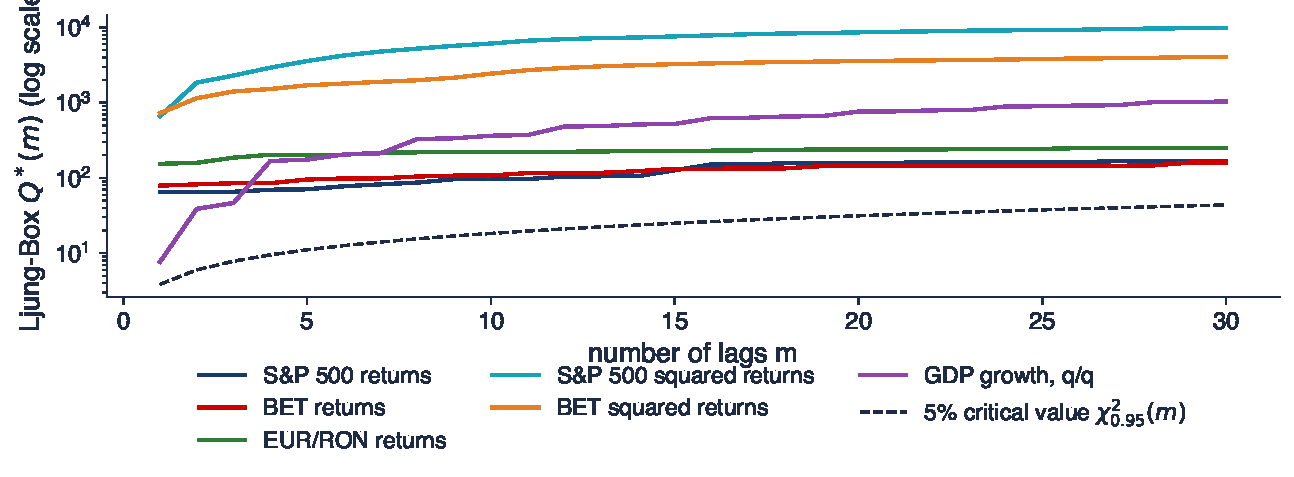
\includegraphics[width=0.97\textwidth,height=0.60\textheight,keepaspectratio]{tsa_ch1_lb_stats.pdf}
\end{center}
\vspace{-0.25cm}
\begin{itemize}
    \item $Q^*(m)$ for $m = 1, \dots, 30$ (log scale) against the 5\% critical value $\chi^2_{0.95}(m)$ (dashed)
\end{itemize}
\quantlet{TSA\_ch1\_portmanteau}{\qlurl{TSA_ch1_portmanteau}}
\end{frame}

\begin{frame}{Interpreting the Ljung--Box statistics}
\itemsize{\footnotesize}
\begin{center}
\scriptsize
\begin{tabular}{lrrrrr}
\toprule
Series & $T$ & $\hat\rho(1)$ & $\hat\rho(4)$ & $Q^*(10)$ & p \\
\midrule
S\&P 500, daily returns & 6\,714 & $\ensuremath{-}0.10$ & $\ensuremath{-}0.03$ & 96.3 & $<$\,0.001 \\
S\&P 500, squared returns & 6\,714 & $0.31$ & $0.31$ & 6132.8 & $<$\,0.001 \\
BET, daily returns & 6\,670 & $0.11$ & $\ensuremath{-}0.01$ & 108.0 & $<$\,0.001 \\
BET, squared returns & 6\,670 & $0.33$ & $0.13$ & 2440.0 & $<$\,0.001 \\
EUR/RON, daily returns & 5\,352 & $0.17$ & $\ensuremath{-}0.06$ & 221.7 & $<$\,0.001 \\
GDP Romania, q/q growth & 125 & $\ensuremath{-}0.24$ & $0.96$ & 364.8 & $<$\,0.001 \\
GDP Romania, y/y growth & 122 & $0.63$ & $0.03$ & 75.0 & $<$\,0.001 \\
HICP Romania, monthly inflation & 260 & $0.40$ & $0.12$ & 126.7 & $<$\,0.001 \\
Nile, yearly flow & 100 & $0.50$ & $0.24$ & 88.1 & $<$\,0.001 \\
Sunspots, yearly & 309 & $0.82$ & $\ensuremath{-}0.28$ & 627.4 & $<$\,0.001 \\
\bottomrule
\end{tabular}
\end{center}
\begin{itemize}
    \item Every series rejects white noise; for the squared returns the statistic is tens of times larger than for the returns
    \item Rejection says only that \textbf{some} correlation exists; the ACF shows where (GDP: lag 4, the season)
\end{itemize}
\end{frame}

\begin{frame}{Recap: Portmanteau tests}
\itemsize{\small}
\begin{itemize}
    \item $Q(m) = T\sum\hat\rho(h)^2$, $Q^*(m) = T(T + 2)\sum\hat\rho(h)^2/(T - h)$; both $\approx \chi^2(m)$ under white noise
    \item Ljung--Box has better size in small samples; keep $m$ well below $T$
    \item A rejection is a signal to model, not a model; under GARCH effects the test of returns rejects too often
\end{itemize}
\end{frame}


%=============================================================================
\section{Transformations}
%=============================================================================

\begin{frame}{Reasons to transform a series}
\itemsize{\small}
\begin{itemize}
    \item Goals
    \begin{itemize}
        \item stabilise the variance (seasonal swings that grow with the level)
        \item turn exponential growth into a linear trend
        \item remove a stochastic trend or a seasonal pattern (differencing)
    \end{itemize}
    \item \textbf{Logarithm}: $\ln Y_t$; its difference is the growth rate in continuous terms
    \begin{itemize}
        \item $100\,\Delta\ln Y_t \approx$ percentage change for small changes: $\ln 1.03 = 0.0296$, about 3\%
        \item not for large ones: $\ln 1.30 = 0.262$, $\ln 0.70 = \ensuremath{-}0.357$; log changes add up over time, percentages do not
    \end{itemize}
    \item Order of operations for a trending, seasonal, positive series
    \begin{itemize}
        \item first the log (variance), then the differences (trend, season); never the other way round
    \end{itemize}
\end{itemize}
\end{frame}

\begin{frame}{Romanian real GDP: log, quarterly and annual growth}
\itemsize{\footnotesize}
\begin{center}
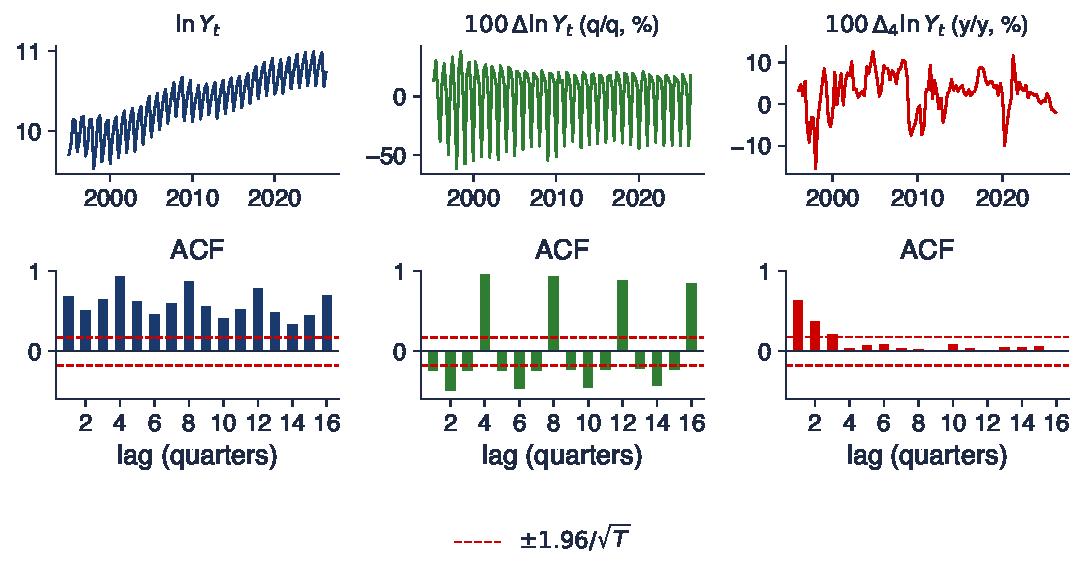
\includegraphics[width=0.97\textwidth,height=0.64\textheight,keepaspectratio]{tsa_ch1_gdp_transform.pdf}
\end{center}
\vspace{-0.25cm}
\begin{itemize}
    \item Quarterly, not seasonally adjusted, 2010 prices (Eurostat), 1995Q1--2026Q2; top: the series; bottom: their sample ACF
\end{itemize}
\quantlet{TSA\_ch1\_transformations}{\qlurl{TSA_ch1_transformations}}
\end{frame}

\begin{frame}{Interpreting the GDP transformations}
\itemsize{\small}
\begin{itemize}
    \item $\ln Y_t$: ACF 0.68 at lag 1 and 0.87 at lag 8, with peaks every 4 quarters: trend and season
    \item $\Delta\ln Y_t$: the trend is gone, the season dominates: $\hat\rho(4) = 0.96$, $\hat\rho(2) = \ensuremath{-}0.49$; standard deviation 27.5\%
    \begin{itemize}
        \item a quarter-on-quarter rate of unadjusted data mostly measures the season
    \end{itemize}
    \item $\Delta_4\ln Y_t$ (annual growth): mean 2.7\%, the ACF dies out after 2--3 quarters ($\hat\rho(1) = 0.63$, $\hat\rho(4) = 0.03$)
    \begin{itemize}
        \item close to stationary, with business-cycle persistence; 2020Q2: $\ensuremath{-}9.9\%$; last quarter: $\ensuremath{-}2.0\%$
    \end{itemize}
\end{itemize}
\end{frame}

\begin{frame}{The Box--Cox transformation}
\itemsize{\small}
\begin{itemize}
    \item \textbf{Definition} \refBC, for $y > 0$: $w = \dfrac{y^\lambda - 1}{\lambda}$ for $\lambda \ne 0$, $w = \ln y$ for $\lambda = 0$
    \begin{itemize}
        \item $\lambda = 1$: no change in shape; $\lambda = 0.5$: square root; $\lambda = 0$: log; $\lambda = -1$: inverse
        \item continuous in $\lambda$: $(y^\lambda - 1)/\lambda \to \ln y$ as $\lambda \to 0$
    \end{itemize}
    \item \textbf{Worked example}: $y = 100$ and $y = 400$
    \begin{itemize}
        \item $\lambda = 0.5$: $w = 18$ and $38$; $\lambda = 0$: $w = 4.605$ and $5.991$
        \item the smaller $\lambda$, the more large values are compressed
    \end{itemize}
    \item Choosing $\lambda$: \refGuerrero, as in \refFPP
    \begin{itemize}
        \item split the series into years; choose $\lambda$ so that $\mathrm{sd}_i/\mathrm{mean}_i^{1-\lambda}$ is as constant as possible across years; $\mathrm{sd}_i$, $\mathrm{mean}_i$: the standard deviation and the mean of year $i$
    \end{itemize}
    \item Forecasts are made for $w$ and transformed back: $y = (\lambda w + 1)^{1/\lambda}$; the back-transformed value is the median, not the mean
\end{itemize}
\end{frame}

\begin{frame}{Box--Cox for Romanian nominal GDP}
\itemsize{\footnotesize}
\begin{center}
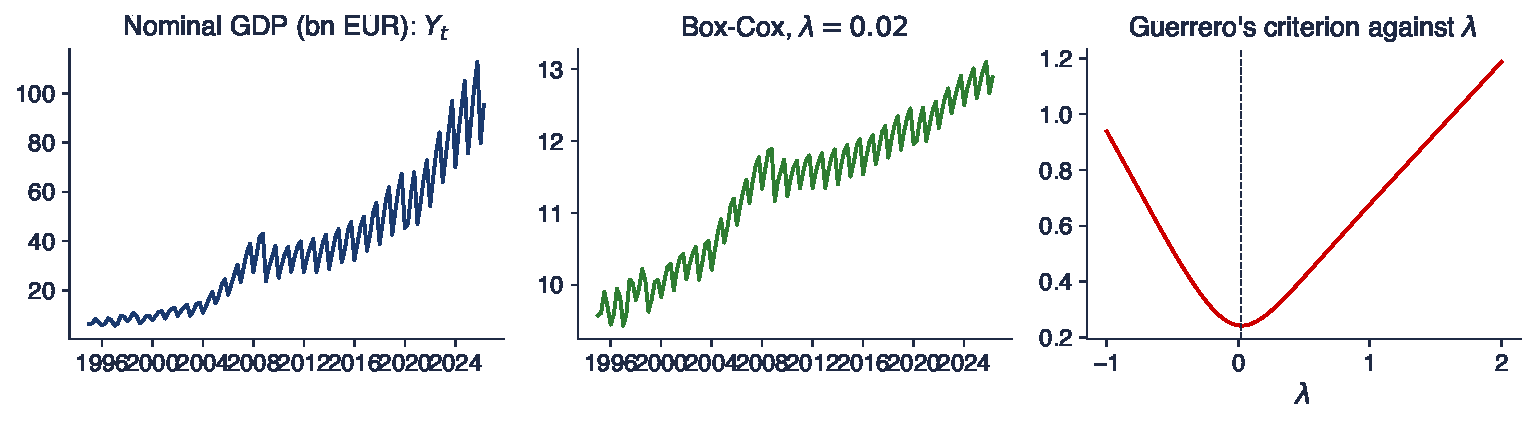
\includegraphics[width=0.97\textwidth,height=0.54\textheight,keepaspectratio]{tsa_ch1_boxcox.pdf}
\end{center}
\vspace{-0.25cm}
\begin{itemize}
    \item Quarterly nominal GDP, not seasonally adjusted, from 6.4 to 95.2 bn EUR; Guerrero's criterion on yearly blocks of 4 quarters
\end{itemize}
\quantlet{TSA\_ch1\_transformations}{\qlurl{TSA_ch1_transformations}}
\end{frame}

\begin{frame}{Interpreting the Box--Cox choice}
\itemsize{\small}
\begin{itemize}
    \item Guerrero's $\hat\lambda = 0.02$: practically the logarithm (criterion 0.243 at $\hat\lambda$, 0.243 at $\lambda = 0$, 0.68 at $\lambda = 1$)
    \begin{itemize}
        \item choose the round, interpretable value: $\lambda = 0$
    \end{itemize}
    \item Why the log fits: the seasonal swing is a stable share of the level, about 39\% in the first five years and 41\% in the last five
    \begin{itemize}
        \item multiplicative seasonality becomes additive after the log
    \end{itemize}
    \item Box--Cox fixes the variance only; the trend and the season still need differencing
\end{itemize}
\end{frame}

\begin{frame}{Over-differencing}
\itemsize{\footnotesize}
\begin{center}
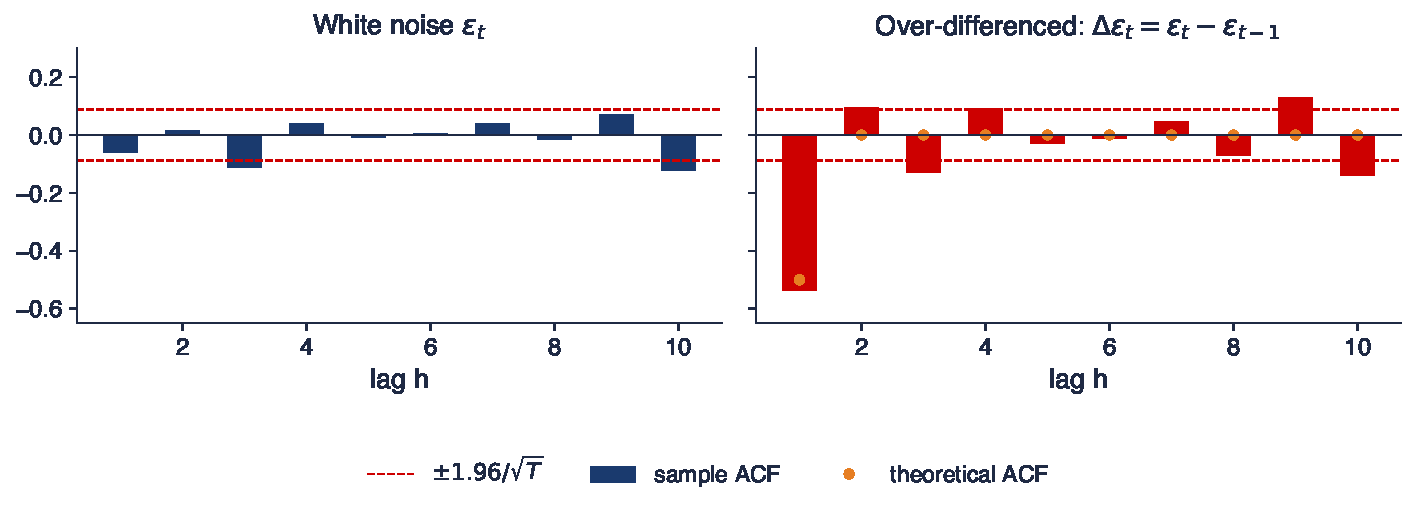
\includegraphics[width=0.97\textwidth,height=0.50\textheight,keepaspectratio]{tsa_ch1_overdiff.pdf}
\end{center}
\vspace{-0.25cm}
\begin{itemize}
    \item Sample ACF of 500 values of white noise (left) and of its first difference (right)
\end{itemize}
\quantlet{TSA\_ch1\_transformations}{\qlurl{TSA_ch1_transformations}}
\end{frame}

\begin{frame}{Interpreting over-differencing}
\itemsize{\small}
\begin{itemize}
    \item $\Delta\varepsilon_t = \varepsilon_t - \varepsilon_{t-1}$ is an MA(1) with $\theta = -1$: $\rho(1) = -1/2$; here $\hat\rho(1) = \ensuremath{-}0.54$
    \begin{itemize}
        \item the variance doubles: 0.95 becomes 2.01
    \end{itemize}
    \item A strongly negative $\hat\rho(1)$, close to $-0.5$, after differencing: a sign that the series did not need it
    \begin{itemize}
        \item the same happens to a trend-stationary series: $\Delta(a + bt + \varepsilon_t) = b + \varepsilon_t - \varepsilon_{t-1}$
    \end{itemize}
    \item Difference as little as needed; \tsachlink{https://danpele.github.io/Time-Series-Analysis/EN/Courses/chapter3_unit_roots_arima_models.pdf}{Chapter 3} gives formal tests for the number of differences
\end{itemize}
\end{frame}

\begin{frame}{Recap: Transformations}
\itemsize{\small}
\begin{itemize}
    \item Log first for positive series whose swings grow with the level; then differences
    \item $100\,\Delta\ln Y_t$: growth in \%; $\Delta_4$, $\Delta_{12}$: annual growth of quarterly and monthly data
    \item Box--Cox with Guerrero's $\lambda$; for Romanian GDP $\hat\lambda \approx 0$, the log
    \item Over-differencing creates $\rho(1) \approx -0.5$ and inflates the variance
\end{itemize}
\end{frame}


%=============================================================================
\section{Two classic series}
%=============================================================================

\begin{frame}{Case study: Yule (1927) and Slutzky (1937)}
\itemsize{\small}
\begin{itemize}
    \item \textbf{Question} of the 1920s: where do the regular cycles of sunspots and of business activity come from?
    \begin{itemize}
        \item the dominant view: hidden periodic components (sums of sine waves), estimated with the periodogram
    \end{itemize}
    \item \refYule: the sunspot number depends on its own last two values plus a random disturbance
    \begin{itemize}
        \item $X_t = \phi_1X_{t-1} + \phi_2X_{t-2} + \varepsilon_t$: the first autoregression; a damped pendulum hit by random shocks
        \item a cycle without any sine wave: the shocks keep it alive, the dynamics give it its period
    \end{itemize}
    \item \refSlutzky: moving sums of purely random numbers (a lottery series) produce smooth, cycle-like waves
    \begin{itemize}
        \item the moving average (MA) process, and a warning: cycles in data may be created by averaging
    \end{itemize}
    \item Legacy: stationary processes built from white noise; \refWold\ unified the two views (Section 4); \refHP, Ch.~3
\end{itemize}
\end{frame}

\begin{frame}{The Nile and the sunspots}
\itemsize{\small}
\begin{columns}[T]
\begin{column}{0.46\textwidth}
\centering
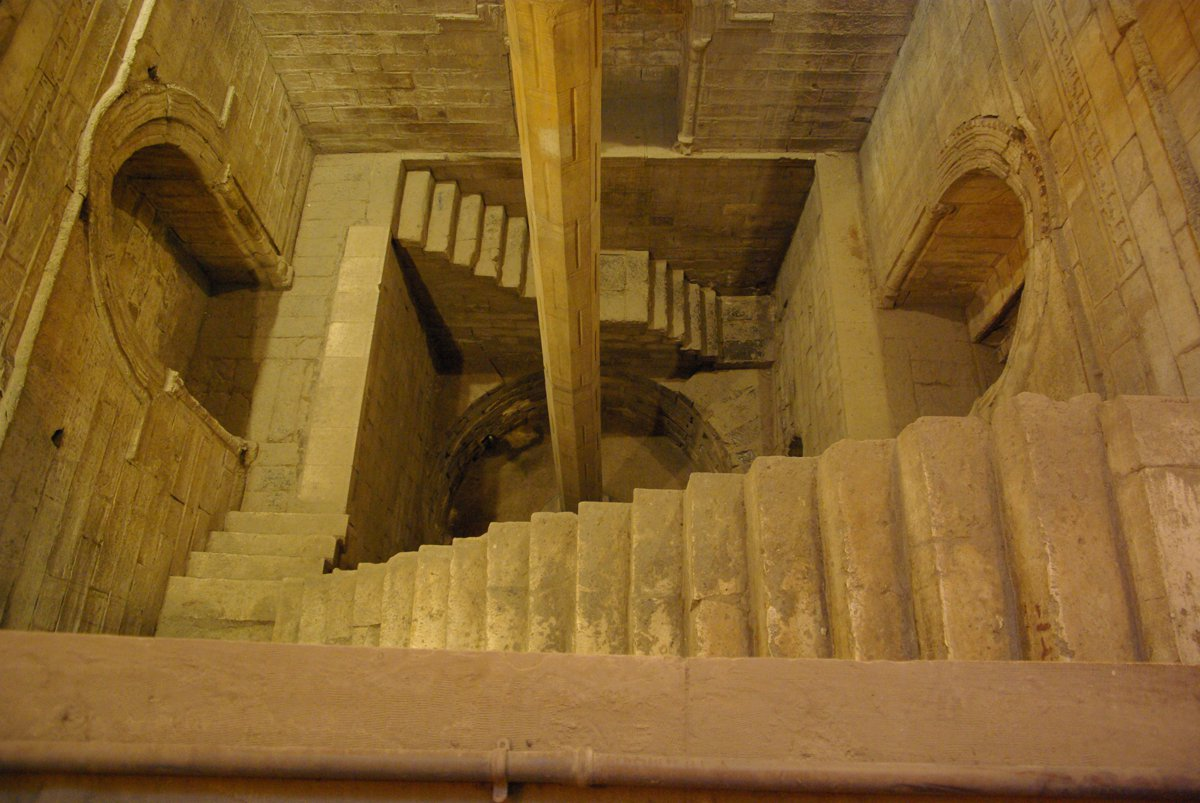
\includegraphics[height=0.44\textheight]{ch1_nilometer_cairo.jpg}\\[1mm]
\imgcap{The Nilometer on Roda Island, Cairo: Nile levels have been recorded here for more than a thousand years}
\imgcredit{https://commons.wikimedia.org/wiki/File:Kairo_Nilometer_BW_1.jpg}{Photo: Berthold Werner (2010); CC BY-SA 3.0; Wikimedia Commons}
\end{column}
\begin{column}{0.50\textwidth}
\begin{itemize}
    \item \textbf{Nile}: yearly flow at Aswan, 1871--1970, 100 observations; a drop around 1898 \refCobb
    \item \textbf{Sunspots}: yearly numbers, 1700--2008, 309 observations; the series that inspired the autoregression \refYule
    \item Both ship with \texttt{statsmodels}; both teach a lesson about reading an ACF
\end{itemize}
\end{column}
\end{columns}
\end{frame}

\begin{frame}{The Nile and the sunspots: series and ACF}
\itemsize{\footnotesize}
\begin{center}
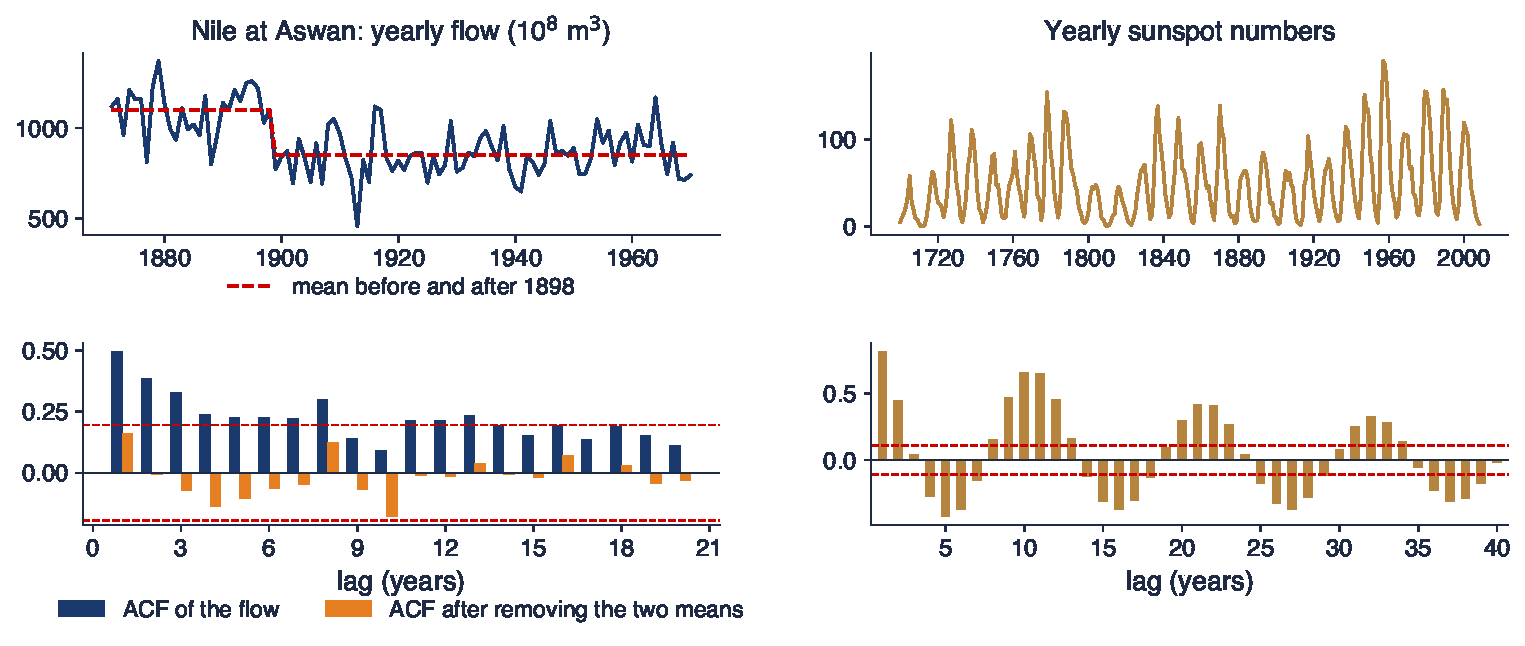
\includegraphics[width=0.97\textwidth,height=0.64\textheight,keepaspectratio]{tsa_ch1_textbook.pdf}
\end{center}
\vspace{-0.25cm}
\begin{itemize}
    \item Left: the Nile flow with its mean before and after 1898, and two ACFs; right: sunspot numbers and their ACF up to lag 40
\end{itemize}
\quantlet{TSA\_ch1\_textbook\_series}{\qlurl{TSA_ch1_textbook_series}}
\end{frame}

\begin{frame}{Interpreting the two classic series}
\itemsize{\small}
\begin{itemize}
    \item Nile: $\hat\rho(1) = 0.50$ and a slow decay; $Q^*(10) = 88.1$ (p $<$\,0.001)
    \begin{itemize}
        \item after removing the two means (1098 and 850): $\hat\rho(1) = 0.16$, $Q^*(10) = 13.0$ (p = 0.225)
        \item a slowly decaying ACF can come from a \textbf{break}, not from persistence or a unit root
    \end{itemize}
    \item Sunspots: a damped wave, minimum $\ensuremath{-}0.43$ at lag 5, peak 0.66 at lag 10
    \begin{itemize}
        \item the solar cycle of about 11 years; a stationary series with a cycle, modelled by \refYule\ with an AR(2)
    \end{itemize}
    \item Read an ACF together with the plot of the series and with what you know about how the data were produced
\end{itemize}
\end{frame}

\begin{frame}{Recap: Two classic series}
\itemsize{\small}
\begin{itemize}
    \item Slow ACF decay has several causes: unit root, strong persistence, structural break
    \item Cycles appear as damped waves in the ACF
\end{itemize}
\end{frame}


%=============================================================================
\section{Possible contribution of AI}
%=============================================================================

\begin{frame}{Possible contribution of AI}
\itemsize{\small}
\begin{itemize}
    \item \textbf{Code}: a first draft of a script that downloads a series, plots it with its ACF and PACF, and runs Ljung--Box for several $m$
    \item \textbf{Explanation}: a second explanation of a definition, or of why a correlogram looks as it does
    \item \textbf{Exploration}: the same diagnostics on many series at once (all BVB stocks, all EU inflation rates)
    \item Example prompt
    \begin{itemize}
        \item \aiprompt{Write Python code that loads the Romanian monthly HICP from Eurostat, computes 100 times the monthly log difference since 2005, plots the series with its ACF and PACF up to lag 36, and reports the Ljung-Box statistic for m = 12 and m = 24.}
    \end{itemize}
\end{itemize}
\end{frame}

\begin{frame}{Checks you must run}
\itemsize{\small}
\begin{itemize}
    \item The divisor of $\hat\gamma(h)$ ($T$, not $T - h$) and whether lag 0 is included in the plot
    \item Which bands are drawn: $\pm 1.96/\sqrt{T}$ or Bartlett's MA bands; they answer different questions
    \item That Ljung--Box is applied to the stationary transformation, not to the level; and with $m - p - q$ degrees of freedom on residuals
    \item That ``significant'' is not read as ``large'' or ``profitable''
    \item Dates, frequencies and units of the data (seasonally adjusted or not, index base, percent or decimals)
    \item Every cited reference: it must exist; check the DOI
\end{itemize}
\end{frame}


%=============================================================================
\section{Summary}
%=============================================================================

\begin{frame}{Key takeaways}
\itemsize{\small}
\begin{itemize}
    \item A time series is one path of a stochastic process; inference from one path needs stationarity and ergodicity
    \item Weak stationarity: constant mean and an autocovariance that depends only on the lag
    \item White noise (weak, i.i.d., Gaussian) is the building block; the random walk is its cumulative sum and is not stationary
    \item Sample ACF and PACF with $\pm 1.96/\sqrt{T}$ bands; Ljung--Box tests many lags jointly
    \item Real series need transformations: log or Box--Cox for the variance, differences for trend and season
    \item Returns: nearly uncorrelated, but their squares are strongly correlated
\end{itemize}
\end{frame}

\begin{frame}{Key formulas}
\itemsize{\small}
{\renewcommand{\arraystretch}{1.4}\begin{center}
\scriptsize
\begin{tabular}{ll}
\toprule
\textbf{Quantity} & \textbf{Formula} \\
\midrule
Autocovariance, ACF & $\gamma(h) = \mathrm{Cov}(X_t, X_{t+h})$, \quad $\rho(h) = \gamma(h)/\gamma(0)$ \\
MA(1) & $\gamma(0) = \sigma^2(1 + \theta^2)$, \quad $\rho(1) = \theta/(1 + \theta^2)$, \quad $\rho(h) = 0$, $|h| \ge 2$ \\
AR(1) & $\gamma(0) = \sigma^2/(1 - \phi^2)$, \quad $\rho(h) = \phi^{|h|}$ \\
Random walk & $\mathrm{Var}(X_t) = t\sigma^2$, \quad $\mathrm{Cov}(X_t, X_s) = \min(t, s)\,\sigma^2$ \\
Wold & $X_t = \sum_{j \ge 0}\psi_j\varepsilon_{t-j} + \eta_t$, \quad $\sum_j\psi_j^2 < \infty$ \\
Sample ACF & $\hat\rho(h) = \sum_{t=1}^{T-h}(x_t - \bar x)(x_{t+h} - \bar x)/\sum_{t=1}^{T}(x_t - \bar x)^2$, \quad $\pm 1.96/\sqrt{T}$ \\
PACF & $\phi_{11} = \rho(1)$, \quad $\phi_{22} = (\rho(2) - \rho(1)^2)/(1 - \rho(1)^2)$ \\
Ljung--Box & $Q^*(m) = T(T + 2)\sum_{h=1}^{m}\hat\rho(h)^2/(T - h) \sim \chi^2(m)$ \\
Box--Cox & $w = (y^\lambda - 1)/\lambda$, \quad $w = \ln y$ ($\lambda = 0$) \\
\bottomrule
\end{tabular}
\end{center}
}
\end{frame}

\begin{frame}{Self-assessment}
\itemsize{\small}
\begin{itemize}
    \item \textbf{Question}: $X_t = \varepsilon_t - 0.5\varepsilon_{t-1}$, $\sigma^2 = 4$. What are $\gamma(0)$ and $\rho(1)$?
    \begin{itemize}
        \item \textbf{Answer}: $\gamma(0) = 4 \times 1.25 = 5$; $\rho(1) = -0.5/1.25 = -0.4$
    \end{itemize}
    \item \textbf{Question}: a correlogram of 40 lags of a series with $T = 400$ shows two bars just outside $\pm 0.098$. Is the series correlated?
    \begin{itemize}
        \item \textbf{Answer}: not necessarily: about 2 of 40 bars cross by chance; run Ljung--Box
    \end{itemize}
    \item \textbf{Question}: after differencing, $\hat\rho(1) = -0.48$ and nothing else is significant. What does this suggest?
    \begin{itemize}
        \item \textbf{Answer}: over-differencing: the original series was probably already stationary
    \end{itemize}
    \item Next: \tsachlink{https://danpele.github.io/Time-Series-Analysis/EN/Courses/chapter2_arma_models.pdf}{Chapter 2}, ARMA models: identification with the ACF and PACF, estimation, diagnostics and forecasts
\end{itemize}
\end{frame}


%=============================================================================
\section{References}
%=============================================================================

\begin{frame}{References (1/2)}
\itemsize{\scriptsize}
\begin{itemize}
    \item Bartlett, M. S. (1946). On the theoretical specification and sampling properties of autocorrelated time-series. \textit{Supplement to the Journal of the Royal Statistical Society}, 8(1), 27--41. \href{https://doi.org/10.2307/2983611}{doi:10.2307/2983611}
    \item Box, G. E. P., \& Cox, D. R. (1964). An analysis of transformations. \textit{Journal of the Royal Statistical Society: Series B}, 26(2), 211--243. \href{https://doi.org/10.1111/j.2517-6161.1964.tb00553.x}{doi:10.1111/j.2517-6161.1964.tb00553.x}
    \item Box, G. E. P., \& Pierce, D. A. (1970). Distribution of residual autocorrelations in autoregressive-integrated moving average time series models. \textit{Journal of the American Statistical Association}, 65(332), 1509--1526. \href{https://doi.org/10.1080/01621459.1970.10481180}{doi:10.1080/01621459.1970.10481180}
    \item Brockwell, P. J., \& Davis, R. A. (1991). \textit{Time Series: Theory and Methods} (2nd ed.). Springer. \href{https://doi.org/10.1007/978-1-4419-0320-4}{doi:10.1007/978-1-4419-0320-4}
    \item Brockwell, P. J., \& Davis, R. A. (2016). \textit{Introduction to Time Series and Forecasting} (3rd ed.). Springer. \href{https://doi.org/10.1007/978-3-319-29854-2}{doi:10.1007/978-3-319-29854-2}
    \item Cobb, G. W. (1978). The problem of the Nile: Conditional solution to a changepoint problem. \textit{Biometrika}, 65(2), 243--251. \href{https://doi.org/10.1093/biomet/65.2.243}{doi:10.1093/biomet/65.2.243}
    \item Guerrero, V. M. (1993). Time-series analysis supported by power transformations. \textit{Journal of Forecasting}, 12(1), 37--48. \href{https://doi.org/10.1002/for.3980120104}{doi:10.1002/for.3980120104}
    \item Hamilton, J. D. (1994). \textit{Time Series Analysis}. Princeton University Press. \href{https://doi.org/10.2307/j.ctv14jx6sm}{doi:10.2307/j.ctv14jx6sm}
\end{itemize}
\end{frame}

\begin{frame}{References (2/2)}
\itemsize{\scriptsize}
\begin{itemize}
    \item Huang, C., \& Petukhina, A. (2022). \textit{Applied Time Series Analysis and Forecasting with Python}. Springer. \href{https://doi.org/10.1007/978-3-031-13584-2}{doi:10.1007/978-3-031-13584-2}
    \item Hyndman, R. J., \& Athanasopoulos, G. (2021). \textit{Forecasting: Principles and Practice} (3rd ed.). OTexts. \href{https://otexts.com/fpp3/}{otexts.com/fpp3}
    \item Khintchine, A. (1934). Korrelationstheorie der stationären stochastischen Prozesse. \textit{Mathematische Annalen}, 109, 604--615. \href{https://doi.org/10.1007/BF01449156}{doi:10.1007/BF01449156}
    \item Ljung, G. M., \& Box, G. E. P. (1978). On a measure of lack of fit in time series models. \textit{Biometrika}, 65(2), 297--303. \href{https://doi.org/10.1093/biomet/65.2.297}{doi:10.1093/biomet/65.2.297}
    \item Shumway, R. H., \& Stoffer, D. S. (2017). \textit{Time Series Analysis and Its Applications} (4th ed.). Springer. \href{https://doi.org/10.1007/978-3-319-52452-8}{doi:10.1007/978-3-319-52452-8}
    \item Slutzky, E. (1937). The summation of random causes as the source of cyclic processes. \textit{Econometrica}, 5(2), 105--146. \href{https://doi.org/10.2307/1907241}{doi:10.2307/1907241}
    \item Wold, H. (1938). \textit{A Study in the Analysis of Stationary Time Series}. Almqvist \& Wiksell. \href{https://archive.org/details/in.ernet.dli.2015.262214}{archive.org}
    \item Yule, G. U. (1927). On a method of investigating periodicities in disturbed series, with special reference to Wolfer's sunspot numbers. \textit{Philosophical Transactions of the Royal Society A}, 226, 267--298. \href{https://doi.org/10.1098/rsta.1927.0007}{doi:10.1098/rsta.1927.0007}
\end{itemize}
\end{frame}

\end{document}
